% XeLaTeX document
\documentclass[12pt,a4paper]{article}
% Редактируем: конфигурация, личные настройки: имя, название предмета и пр. для титульной страницы и метаданных документа здесь
\newcommand{\university}{Санкт-Петербургский политехнический университет Петра Великого}
\newcommand{\faculty}{Институт компьютерных наук и технологий}
\newcommand{\department}{Высшая школа интеллектуальный систем и суперкомпьютерных технологий}
\newcommand{\city}{Санкт-Петербург}
\newcommand{\docname}{Отчёт по лабораторным работам}
\newcommand{\subject}{Телекоммуникационные технологии}
\newcommand{\tutorname}{Н. В. Богач}
\newcommand{\studentname}{Е. В. Бурков}
\newcommand{\group}{3530901/90201}

% Не редактируем: используемые пакеты
% настройка кодировки, шрифтов и русского языка
\usepackage{fontspec}
\usepackage{polyglossia}

% рабочие ссылки в документе
\usepackage{hyperref}

% графика
\usepackage{graphicx}
\usepackage{tikz}

% поворот страницы
\usepackage{pdflscape}

% качественные листинги кода
\usepackage{minted}
\usepackage{lstfiracode}

\usepackage{listings}


\usepackage{xcolor}
%New colors defined below
\definecolor{codegreen}{rgb}{0,0.6,0}
\definecolor{codegray}{rgb}{0.5,0.5,0.5}
\definecolor{codepurple}{rgb}{0.58,0,0.82}
\definecolor{backcolour}{rgb}{0.95,0.95,0.92}

%Code listing style named "mystyle"
\lstdefinestyle{mystyle}{
  backgroundcolor=\color{backcolour}, commentstyle=\color{codegreen},
  keywordstyle=\color{magenta},
  numberstyle=\tiny\color{codegray},
  stringstyle=\color{codepurple},
  basicstyle=\ttfamily\footnotesize,
  breakatwhitespace=false,         
  breaklines=true,                 
  captionpos=b,                    
  keepspaces=false,                 
  numbers=left,                    
  numbersep=5pt,                  
  showspaces=false,                
  showstringspaces=false,
  showtabs=false,                  
  tabsize=2
}



% отключение копирования номеров строк из листинга, работает не во всех просмотрщиках (в Adobe Reader работает)
\usepackage{accsupp}
\newcommand\emptyaccsupp[1]{\BeginAccSupp{ActualText={}}#1\EndAccSupp{}}
\let\theHFancyVerbLine\theFancyVerbLine
\def\theFancyVerbLine{\rmfamily\tiny\emptyaccsupp{\arabic{FancyVerbLine}}}

% библиография
\bibliographystyle{templates/gost-numeric.bbx}
\usepackage{csquotes}
\usepackage[parentracker=true,backend=biber,hyperref=true,bibencoding=utf8,style=numeric-comp,language=auto,autolang=other,citestyle=gost-numeric,defernumbers=true,bibstyle=gost-numeric,sorting=ntvy]{biblatex}

% установка полей
\usepackage{geometry}

% нумерация картинок по секциям
\usepackage{chngcntr}

% дополнительные команды для таблиц
\usepackage{booktabs}

% для заголовков
\usepackage{caption}
\usepackage{titlesec}
\usepackage[dotinlabels]{titletoc}

% разное для математики
\usepackage{amsmath, amsfonts, amssymb, amsthm, mathtools}

% водяной знак на документе, см. main.tex
\usepackage[printwatermark]{xwatermark}

% Не редактируем: параметры используемых пакетов и не только
% настройки polyglossia
\setdefaultlanguage{russian}
\setotherlanguage{english}

% локализация
\addto\captionsrussian{
	\renewcommand{\figurename}{Рисунок}%
	\renewcommand{\partname}{Глава}
	\renewcommand{\contentsname}{\centerline{Содержание}}
	\renewcommand{\listingscaption}{Листинг}
}

% основной шрифт документа
\setmainfont{CMU Serif}
\newfontfamily\cyrillicfont{CMU Serif}[Script=Cyrillic]

% перечень использованных источников
\addbibresource{refs.bib}

% настройка полей
\geometry{top=2cm}
\geometry{bottom=2cm}
\geometry{left=2cm}
\geometry{right=2cm}
\geometry{bindingoffset=0cm}

% настройка ссылок и метаданных документа
\hypersetup{unicode=true,colorlinks=true,linkcolor=red,citecolor=green,filecolor=magenta,urlcolor=cyan,
	pdftitle={\docname},
	pdfauthor={\studentname},
	pdfsubject={\subject},
	pdfcreator={\studentname},
	pdfproducer={Overleaf},
	pdfkeywords={\subject}
}

% настройка подсветки кода и окружения для листингов
\usemintedstyle{colorful}
\newenvironment{code}{\captionsetup{type=listing}}{}

% шрифт для листингов с лигатурами
\setmonofont{FiraCode-Regular.otf}[
	SizeFeatures={Size=10},
	Path = templates/,
	Contextuals=Alternate
]

% оформления подписи рисунка
\captionsetup[figure]{labelsep = period}

% подпись таблицы
\DeclareCaptionFormat{hfillstart}{\hfill#1#2#3\par}
\captionsetup[table]{format=hfillstart,labelsep=newline,justification=centering,skip=-10pt,textfont=bf}

% путь к каталогу с рисунками
\graphicspath{{fig/}}

% Внесение titlepage в учёт счётчика страниц
\makeatletter
\renewenvironment{titlepage} {
	\thispagestyle{empty}
}
\makeatother

\counterwithin{figure}{section}
\counterwithin{table}{section}

\titlelabel{\thetitle.\quad}

% для удобного конспектирования математики
\mathtoolsset{showonlyrefs=true}
\theoremstyle{plain}
\newtheorem{theorem}{Теорема}[section]
\newtheorem{proposition}[theorem]{Утверждение}
\theoremstyle{definition}
\newtheorem{corollary}{Следствие}[theorem]
\newtheorem{problem}{Задача}[section]
\theoremstyle{remark}
\newtheorem*{nonum}{Решение}

% настоящее матожидание
\newcommand{\MExpect}{\mathsf{M}}

% объявили оператор!
\DeclareMathOperator{\sgn}{\mathop{sgn}}

% перенос знаков в формулах (по Львовскому)
\newcommand*{\hm}[1]{#1\nobreak\discretionary{} {\hbox{$\mathsurround=0pt #1$}}{}}


% водяной знак для обозначения статуса документа
% \newwatermark[allpages,color=red!5,angle=45,scale=3,xpos=0,ypos=0]{DRAFT}
\begin{document}
% Не редактируем: Титульная страница (формируется автоматически из заданной конфигурации)
\begin{titlepage}	% начало титульной страницы

	\begin{center}		% выравнивание по центру

		\large \university \\
		\large \faculty \\
		\large \department \\[6cm]
		% название института, затем отступ 6см

		\huge \subject \\[0.5cm] % название работы, затем отступ 0,5см
		\large \docname \num \\[5.1cm]
		% \large Тема работы\\[5cm]

	\end{center}


	\begin{flushright} % выравнивание по правому краю
		\begin{minipage}{0.25\textwidth} % врезка в половину ширины текста
			\begin{flushleft} % выровнять её содержимое по левому краю

				\large\textbf{Работу выполнил:}\\
				\large \studentname \\
				\large {Группа:} \group \\

				\large \textbf{Преподаватель:}\\
				\large \tutorname

			\end{flushleft}
		\end{minipage}
	\end{flushright}

	\vfill % заполнить всё доступное ниже пространство

	\begin{center}
		\large \city \\
		\large \the\year % вывести дату
	\end{center} % закончить выравнивание по центру

\end{titlepage} % конец титульной страницы

\vfill % заполнить всё доступное ниже пространство


% Не редактируем: Страница содержания (формируется автоматически из section, subsection и пр., указанных в content.tex)
% Содержание
\tableofcontents
\newpage



\lstset{style=mystyle}
% Редактируем: всё остальное: вступление, др. этапы, заключение, приложение
\section{Звуки и сигналы}
\subsection{Упражнение 1}

Скачайте с сайта http://freesound.org , включающий музыку, речь или иные звуки, имеющие четко выраженную высоту. Выделите примерно полусекундный сегмент, в котором высота постоянна. Вычислите и распечатайте спектр выбранного сегмента. Как связаны тембр звука и гармоническая структура, видимая в спектре?


\noindent Используйте high\_pass, low\_pass, и band\_stop для фильтрациитех или иных гармоник. Затем преобразуйте спектры обратно в сигнал и прослушайте его. Как звук соотносится с изменениями, сделанными в спектре?
    

Загружаем звуки игры на пианино, взятые на сайте freesound.org и загруженные на мой репозиторий, после читаем звуки в специальный Wave класс и вырезаем фрагмент.

\begin{lstlisting}[language=Python]
if not os.path.exists('164718__bradovic__piano.wav'):
    !wget https://github.com/wooftown/spbstu-telecom/raw/main/Content/164718__bradovic__piano.wav
wave = read_wave('164718__bradovic__piano.wav')
wave.make_audio()
wave = wave.segment(18.3,0.5)
wave.make_audio()
read_wave('164718__bradovic__piano.wav').plot()
wave.plot()
\end{lstlisting}
    
\begin{figure}[H]
	\begin{center}
		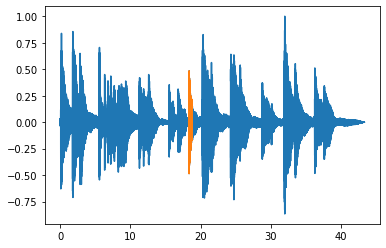
\includegraphics[scale=1]{fig/lab01/lab01_9_0.png}
		\caption{График фрагмента звука}
	\end{center}
\end{figure}

При помощи метода make\_spectrum вычислим спектр звука, и для удобства построим график.
\begin{lstlisting}[language=Python]
spectrum = wave.make_spectrum()
spectrum.plot(high=5000)
\end{lstlisting}

\begin{figure}[H]
	\begin{center}
		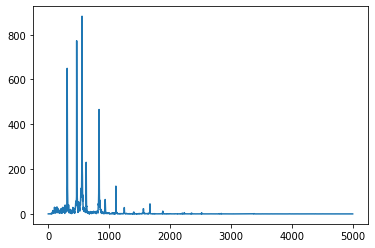
\includegraphics[scale=1]{fig/lab01/lab01_11_0.png}
		\caption{Спектр звука}
	\end{center}
\end{figure}

Можно задать максимальную частоту для графика:

\begin{figure}[H]
	\begin{center}
		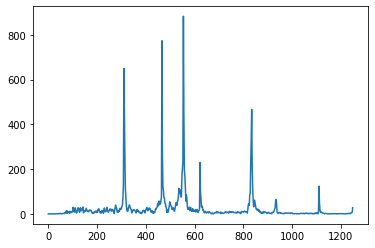
\includegraphics[scale=1]{fig/lab01/lab01_13_0.png}
		\caption{Спектр звука, частота меньше 1250 ГЦ}
	\end{center}
\end{figure}

Для точного понимания какие ноты сыграны выведем список пиков частот в спектре:

\begin{lstlisting}[language=Python]
spectrum.peaks()[:10]
\end{lstlisting}

\begin{lstlisting}
[(882.3500533686324, 554.0),
 (772.8812508117549, 466.0),
 (649.662314039115, 310.0),
 (466.0353893832775, 834.0),
 (455.88324114785496, 312.0),
 (435.6400663619303, 556.0),
 (328.0318016013845, 832.0),
 (260.99365239113706, 314.0),
 (251.02745102094198, 468.0),
 (234.35739758178494, 552.0)]
\end{lstlisting}


Находим соответствие музыкальных нот и частот из пиков:
\begin{itemize}
\item 554.36 Гц - До-диез второй октавы
\item 466.16 Гц - Ля-диез первой октавы
\item 311.13 Гц - Ре-диез первой октавы
\item 830.60 Гц - Соль-диез второй октавы
\end{itemize}
У До-диез второй октавы самая большая амплитуда, поэтому 554.36 Гц - доминирующая частота. Общая воспринимаемая высота звука зависит от основной частоты, тут о
на 311.13 Гц.

Добавим фильтр нижних частот. Все компоненты выше 540 ГЦ будут удалены. (На самом деле можно выбирать на сколько их ослаблять, но я решил на 100\%).

\begin{lstlisting}[language=Python]
spectrum2 = wave.make_spectrum()
spectrum2.low_pass(540)
spectrum2.plot(high=1000)
\end{lstlisting}

\begin{figure}[H]
	\begin{center}
		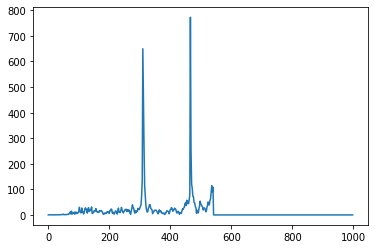
\includegraphics[scale=1]{fig/lab01/lab01_21_0.png}
		\caption{Спект с фильтром нижних частот}
	\end{center}
\end{figure}

Добавим фильтр верхних частот, и ослабим на половину компоненты до 500 Гц.

\begin{lstlisting}[language=Python]
spectrum2.high_pass(500,0.5)
spectrum2.plot(high=1000)
\end{lstlisting}

\begin{figure}[H]
	\begin{center}
		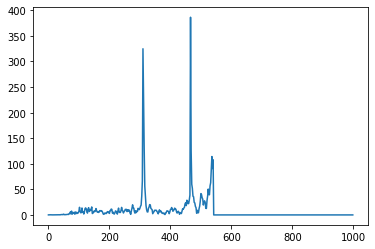
\includegraphics[scale=1]{fig/lab01/lab01_23_0.png}
		\caption{Спект с фильтром верхних частот}
	\end{center}
\end{figure}

Уберём частоты между Ре и Ля.

\begin{lstlisting}[language=Python]
spectrum2.band_stop(320,450)
spectrum2.plot(high=1000)
\end{lstlisting}



\begin{figure}[H]
	\begin{center}
		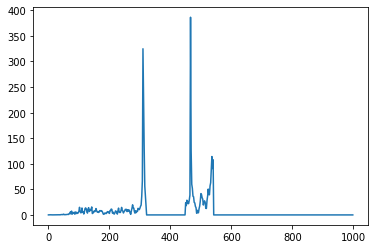
\includegraphics[scale=1]{fig/lab01/lab01_25_0.png}
		\caption{Получившийся спектр}
	\end{center}
\end{figure}

Звучание заметно изменилось из-за изменения доиминирующей частоты (её ампилитуда была уменьшена в 2 раза), но напоминает изначальный отрезок.

\begin{lstlisting}[language=Python]
wave = read_wave('164718__bradovic__piano.wav')
wave = wave.segment(18.3,0.5)
spectrum2 = wave.make_spectrum()
spectrum2.high_pass(500)
spectrum2.plot(high=1000)
\end{lstlisting}

\begin{figure}[H]
	\begin{center}
		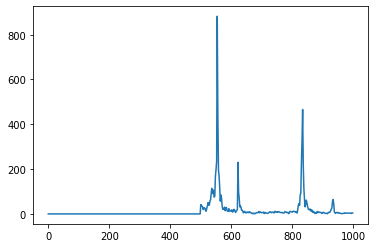
\includegraphics[scale=1]{fig/lab01/lab01_28_0.png}
		\caption{Отфилтрованные нижние компоненты}
	\end{center}
\end{figure}

Отфильтровав нижние частоты звук стал более высоким.

\subsection{Упражнение 2}

Создайте сложный сигнал из объектов SinSignal и CosSignal, суммируя их. Обработайте сигнал для получения wave и прослушайте его. Вычислите Spectrum и распечатайте. Что произойдёт при добавлении частотных компонент, не кратных основным?


Берём два сигнала с частотой одной октавы.
\begin{lstlisting}[language=Python]
from thinkdsp import SinSignal, CosSignal
# https://nch-nch.ru/apps/frequency/
cos_sig1 = CosSignal(freq=784.00,amp=1,offset=0)
sin_sig2 = CosSignal(freq=392.00,amp=0.5,offset=0)
mix = cos_sig1 + sin_sig2
wave = mix.make_wave(duration=1)
wave.make_audio()
\end{lstlisting}

\begin{figure}[H]
	\begin{center}
		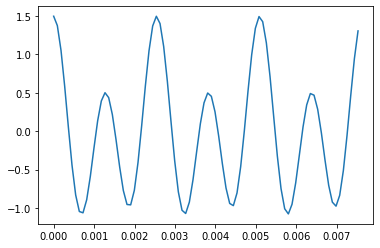
\includegraphics[scale=1]{fig/lab01/lab01_34_0.png}
		\caption{Суммированные сигналы}
	\end{center}
\end{figure}

\begin{lstlisting}[language=Python]
spectrum = wave.make_spectrum()
spectrum.plot(high = 1000)
\end{lstlisting}

\begin{figure}[H]
	\begin{center}
		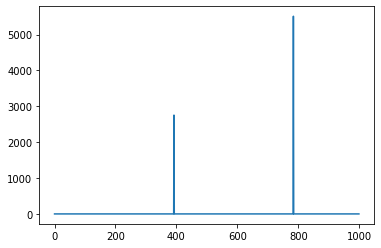
\includegraphics[scale=1]{fig/lab01/lab01_35_0.png}
		\caption{Спектр сигнала}
	\end{center}
\end{figure}

Добавим частоту из другой октавы. Должно получится ужасно для ушей.

\begin{lstlisting}[language=Python]
cos_signal3 = CosSignal(freq = 500, amp=0.25,offset = 0)
mix = mix + cos_signal3
wave = mix.make_wave(duration=1)
wave.make_audio()
\end{lstlisting}

На графике за 7мс не видно цикла.
\begin{figure}[H]
	\begin{center}
		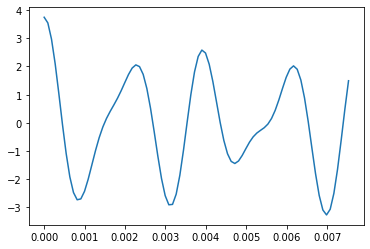
\includegraphics[scale=1]{fig/lab01/lab01_39_0.png}
		\caption{Получившийся сигнал}
	\end{center}
\end{figure}

Действительно, звук очень неприятный.


\subsection{Упражнение 3}

Напишите функцию strech, берущую wave и коэффицент изменения. Она должна ускорять или замедлять сигнал изменением ts и framerate.

\noindent ts - отвечает за моменты выборки сигнала framerate - число выборок в единицу времени.

\noindent Если умножим ts на k, то интервалы между моментами увеличатся в k раз.

\noindent Если framerate поделим на k, то будет меньшее число подвыборок.

\begin{lstlisting}[language=Python]
def stretch(wave, k):
  wave.ts *= k
  wave.framerate /= k
  return wave 
\end{lstlisting}


\subsection{Вывод}
В ходе данной работы было выполнено знакомство с основыми понятиями при работе со звуками и сигналами. При помощи библиотеки thinkDSP можно делать обширный круг взаимодействий с сигналами, как для их создания, так и для их обработки.
\newpage

\section{Гармоники}
\subsection{Упражнение 1}

Пилообразный сигнал линейно нарастает от -1 до 1, а затем резко падает до -1 и повторяется.

\noindent Напишите класс, называемый SawtoothSignal, расширяющий signal и предоставляющий evaluate для оценки пилообразного сигнала.

\noindent Вычислите спектр пилообразного сигнала. Как соотносится его гармоническая структура с тругольными с прямоугольными сигналами?

Напишем класс пилообразного сигнала:

\begin{lstlisting}[language=Python]
class SawtoothSignal(Sinusoid):

  def evaluate(self,ts):
    cycles = self.freq * ts + self.offset / (pi / 2)
    frac, _ = np.modf(cycles)
    u = unbias(frac)
    high, low = abs(max(u)), abs(min(u))
    ys = self.amp * u / max(high,low)
    return ys
\end{lstlisting}

Проверим график:

\begin{lstlisting}[language=Python]
saw_signal = SawtoothSignal(200)
saw_signal.plot()
\end{lstlisting}

\begin{figure}[H]
	\begin{center}
		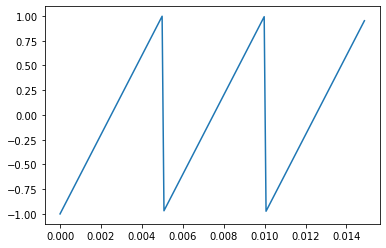
\includegraphics[scale=1]{fig/lab02/lab02_5_0.png}
		\caption{График пилообразного сигнала}
	\end{center}
\end{figure}

Сделаем экземпляр класса Wave для построения спектра сигнала.

\begin{lstlisting}[language=Python]
saw_spectrum = saw_signal.make_wave(duration = 0.5).make_spectrum()
saw_spectrum.plot()
\end{lstlisting}

\begin{figure}[H]
	\begin{center}
		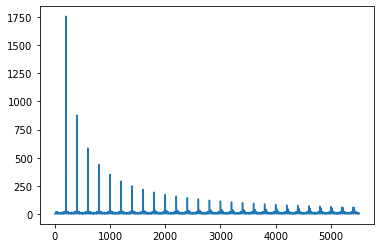
\includegraphics[scale=1]{fig/lab02/lab02_7_0.png}
		\caption{Спектр пилообразного сигнала}
	\end{center}
\end{figure}

Добавим прямоугольный сигнал:

\begin{lstlisting}[language=Python]
from thinkdsp import SquareSignal

squar_signal = SquareSignal(amp = 0.25)
squar_signal.plot()
\end{lstlisting}

\begin{figure}[H]
	\begin{center}
		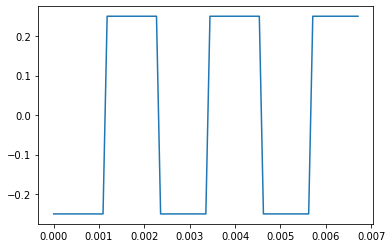
\includegraphics[scale=1]{fig/lab02/lab02_9_0.png}
		\caption{График прямоугольного сигнала}
	\end{center}
\end{figure}

\begin{lstlisting}[language=Python]
squar_spectrum = squar_signal.make_wave().make_spectrum()
squar_spectrum.plot()
\end{lstlisting}

\begin{figure}[H]
	\begin{center}
		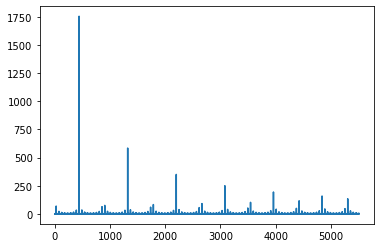
\includegraphics[scale=1]{fig/lab02/lab02_10_0.png}
		\caption{Спектр прямоугольного сигнала}
	\end{center}
\end{figure}

Также добавим треугольный сигнал:

\begin{lstlisting}[language=Python]
from thinkdsp import TriangleSignal

tri_signal = TriangleSignal(amp = 0.5)
tri_signal.plot()
\end{lstlisting}

\begin{figure}[H]
	\begin{center}
		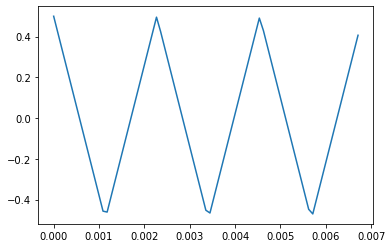
\includegraphics[scale=1]{fig/lab02/lab02_12_0.png}
		\caption{График треугольного сигнала}
	\end{center}
\end{figure}

\begin{lstlisting}[language=Python]
tri_spectrum = tri_signal.make_wave().make_spectrum()
tri_spectrum.plot()
\end{lstlisting}

\begin{figure}[H]
	\begin{center}
		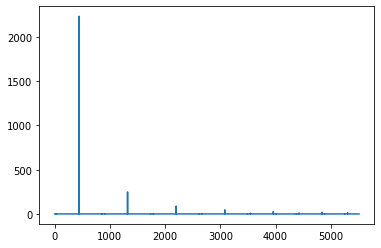
\includegraphics[scale=1]{fig/lab02/lab02_13_0.png}
		\caption{Спектр треугольного сигнала}
	\end{center}
\end{figure}

По сравнению с квадратным сигналом, пилообразный включает в себя четные и нечётные гармоники. Но оба сигнала снижают амплитуду обратно пропорциально частоте.
По сравнению с треугольным сигналом, треугольный сигнал падает $1/f^2$, а пилообразный $1/f$.

\subsection{Упражнение 2}

Создайте прямугольный сигнал 1100 Гц и вычислите wave с выборками 10 000 кадров в секунду. Постройте спектр и убедитесь, что большинство гармоник "завёрнуты" из-за биений, слышно ли последствия этого при проигрывании?

\begin{lstlisting}[language=Python]
square_signal = SquareSignal(freq=1500)
square_wave = square_signal.make_wave(duration = 1, framerate = 10000)
square_wave.make_spectrum().plot()
\end{lstlisting}

\begin{figure}[H]
	\begin{center}
		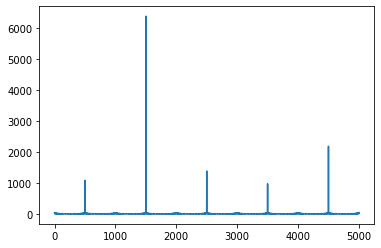
\includegraphics[scale=1]{fig/lab02/lab02_16_0.png}
		\caption{Спектр сигнала с биениями}
	\end{center}
\end{figure}

По спекторграмме видим, что из-за выбранного фреймрейта 10000 у нас начинаются биения. Сигналы больших частот закольцовываются вокруг 5000Гц и 0Гц.

Когда мы слушаем получившийся звук, мы слышим основную частоту на 500Гц.

\begin{lstlisting}[language=Python]
s1 = square_wave.make_spectrum()
s1.high_pass(1000)
s1.plot()
\end{lstlisting}

\begin{figure}[H]
	\begin{center}
		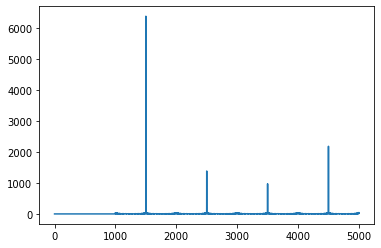
\includegraphics[scale=1]{fig/lab02/lab02_20_0.png}
		\caption{Спектр сигнала с фильтром}
	\end{center}
\end{figure}

Звук отличается, значит действительно, мы слышим звук частотой 500Гц.

\subsection{Упражнение 3}

Возьмите объект спектра spectrum, и выведите первые несколько значений spectrum.fs, вы увидите, что частоты начинаются с нуля. Итак, «spectrum.hs[0]» — это величина компонента с частотой 0. Но что это значит?

\noindent Попробуйте этот эксперимент:

1. Сделать треугольный сигнал с частотой 440 и создать Волну длительностью 0,01 секунды. Постройте форму волны.

2. Создайте объект Spectrum и напечатайте spectrum.hs[0]. Каковы амплитуда и фаза этой составляющей?

3. Установите spectrum.hs[0] = 100. Создайте волну из модифицированного спектра и выведите ее. Как эта операция влияет на форму сигнала?


\begin{lstlisting}[language=Python]
trian_signal = TriangleSignal(freq=440)
trian_wave = trian_signal.make_wave(duration = 0.01)
trian_wave.plot()
\end{lstlisting}

\begin{figure}[H]
	\begin{center}
		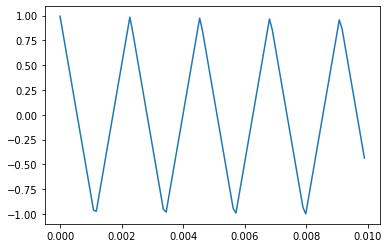
\includegraphics[scale=1]{fig/lab02/lab02_24_0.png}
		\caption{График сигнала}
	\end{center}
\end{figure}

Проверим что лежит в 0 элементе чисел спекторграммы

\begin{lstlisting}[language=Python]
trian_spectrum = trian_wave.make_spectrum()
trian_spectrum.hs[0]
\end{lstlisting}

\begin{lstlisting}
(1.0436096431476471e-14+0j)
\end{lstlisting}
Видим комплексное число, с 0 мнимой частью. Сам элемент очень близок к нулю.

\begin{lstlisting}[language=Python]
trian_spectrum.hs[0] = 100
trian_wave = trian_spectrum.make_wave()
trian_wave.plot()
\end{lstlisting}

\begin{figure}[H]
	\begin{center}
		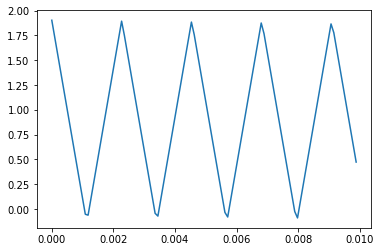
\includegraphics[scale=1]{fig/lab02/lab02_28_0.png}
		\caption{График сигнала с изменённым нулевым числом спекторграммы}
	\end{center}
\end{figure}

Можно заметить, что сигнал сместился по вертикали вверх. Следовательно от первого элемента зависит смещение сигнала. Т.к. сначала элемент был близок к нулю, то нулевой элемент это сигнал без смещения.

\subsection{Упражнение 4}

Напишите функцию, которая принимает Spectrum в качестве параметра и модифицирует его, деля каждый элемент hs на соответствующую частоту из fs. Протестируйте свою функцию, используя один из файлов WAV в репозитории или любой объект Wave.

1. Рассчитайте спектр и начертите его.

2. Измените спектр, используя свою функцию, и снова начертите его.

3. Сделать волну из модифицированного Spectrum и прослушать ее. Как эта операция влияет на сигнал?


Исходя из последнего пункта первый элемент очень близок к нулю. Поэтому на него делить не надо, а то получим очень большие значения (на самом деле я понял это после запуска программы из-за ошибок при делении на ноль).

\begin{lstlisting}[language=Python]
def spectrum_divider(spectrum):
    spectrum.hs[1:] /= spectrum.fs[1:]
    spectrum.hs[0] = 0
\end{lstlisting}

\begin{lstlisting}[language=Python]
if not os.path.exists('164718__bradovic__piano.wav'):
    !wget https://github.com/wooftown/spbstu-telecom/raw/main/Content/164718__bradovic__piano.wav
    
wave = read_wave('164718__bradovic__piano.wav').segment(18.3,0.5)
wave.make_audio()
wave.make_spectrum().plot(high = 5000)
\end{lstlisting}

\begin{figure}[H]
	\begin{center}
		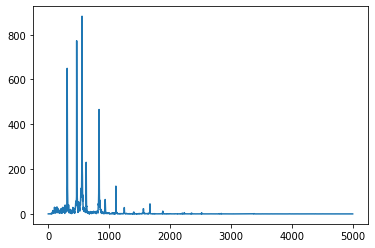
\includegraphics[scale=1]{fig/lab02/lab02_35_0.png}
		\caption{Спектр сигнала}
	\end{center}
\end{figure}

\begin{lstlisting}[language=Python]
sp = wave.make_spectrum()
spectrum_divider(sp)
sp.plot(high = 5000)
\end{lstlisting}

\begin{figure}[H]
	\begin{center}
		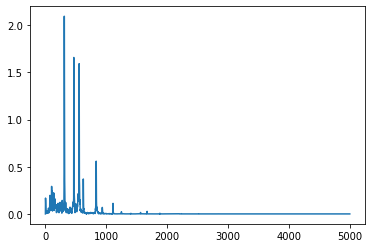
\includegraphics[scale=1]{fig/lab02/lab02_36_0.png}
		\caption{Спектр изменённого сигнала}
	\end{center}
\end{figure}

Видим. что ампилутуда очень поменялась, а частоты стоящие ближе к 0 Гц стали больше, чем следующие, что понятно. На выходе получилось, что полученный звук звучит более чисто, из-за фильтрации высоких частот.

\subsection{Упражнение 5}

Треугольные и прямоугольные волны имеют только нечетные гармоники; пилообразная волна имеет как четные, так и нечетные гармоники. Гармоники прямоугольной и пилообразной волн затухают пропорционально $1/f$; гармоники треугольной волны затухают как $1/f^2$. Можете ли вы найти форму волны, в которой четные и нечетные гармоники затухают как $1/f^2$?

\noindent Подсказка: есть два способа подойти к этому: вы можете построить нужный сигнал путем сложения синусоид, или вы может начаться с сигнала, похожего на то, что вы хотите, и изменить его.


\noindent Не зря мы писали предыдущую функцию, поэтому возьмём пилообразный сигнал который имеет и четные и нечётные гармоники, а потом применим нашу функцию.

\begin{lstlisting}[language=Python]
saw_signal = SawtoothSignal(500)
saw_spectrum = saw_signal.make_wave().make_spectrum()
saw_spectrum.plot()
\end{lstlisting}

\begin{figure}[H]
	\begin{center}
		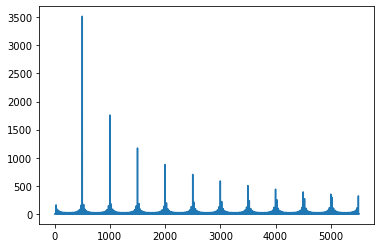
\includegraphics[scale=1]{fig/lab02/lab02_42_0.png}
		\caption{Спектр пилообразного сигнала}
	\end{center}
\end{figure}

\begin{lstlisting}[language=Python]
saw_spectrum1 =  saw_signal.make_wave().make_spectrum()
spectrum_divider(saw_spectrum1)
saw_spectrum1.plot()
\end{lstlisting}

\begin{figure}[H]
	\begin{center}
		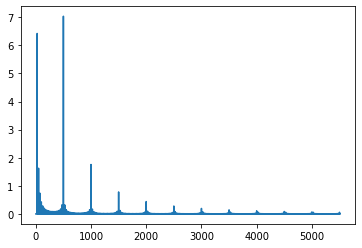
\includegraphics[scale=1]{fig/lab02/lab02_43_0.png}
		\caption{Спектр пилообразного сигнала}
	\end{center}
\end{figure}

Тут получилось, что амплитуда у 0 слишком большая, исправим изменив параметры.

\begin{lstlisting}[language=Python]
saw_signal = SawtoothSignal(freq=freq)
saw_wave = saw_signal.make_wave(duration=1, framerate=10000)
saw_spectrum = saw_wave.make_spectrum()
saw_spectrum.plot()
saw_spectrum1 = saw_wave.make_spectrum()
spectrum_divider(saw_spectrum1)
saw_spectrum1.plot()
\end{lstlisting}

\begin{figure}[H]
	\begin{center}
		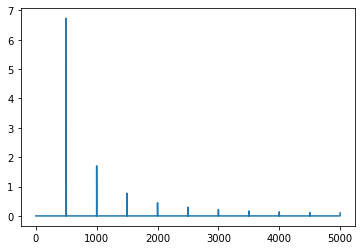
\includegraphics[scale=1]{fig/lab02/lab02_47_0.png}
		\caption{Спектр необходимого сигнала}
	\end{center}
\end{figure}

Теперь нам интересно какой получился график:

\begin{lstlisting}[language=Python]
saw_spectrum1.make_wave().segment(duration = 0.005).plot()
\end{lstlisting}

\begin{figure}[H]
	\begin{center}
		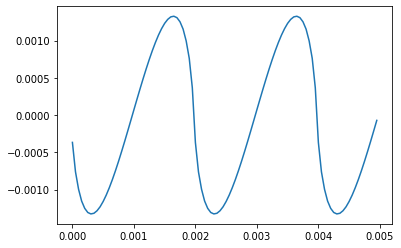
\includegraphics[scale=1]{fig/lab02/lab02_49_0.png}
		\caption{График необходимого сигнала}
	\end{center}
\end{figure}

Сигнал немного напоминает синусойду, но она как-будто немного наклонена.

\subsection{Вывод}

В данной работе были исследованы некоторые виды сигналов. Были рассмотрены спектры и гармонические структуры сигналов. Также в одном из пунктов были замечены биения и мы проверили их действие на звук.
\newpage

\section{Непериодические сигналы}
\subsection{Упражнение 1}

Запустите и прослушайте примеры в файле chap03.ipynb. В примере с утечкой попробуйте заменить окно Хэмминга одним из других окон, предоставляемых NumPy, и посмотрите, как они влияют на утечку.

\begin{lstlisting}[language=Python]
signal = SinSignal(freq=440)
duration = signal.period * 30.25
wave = signal.make_wave(duration)
spectrum = wave.make_spectrum()
spectrum.plot(high=880)
\end{lstlisting}

\begin{figure}[H]
	\begin{center}
		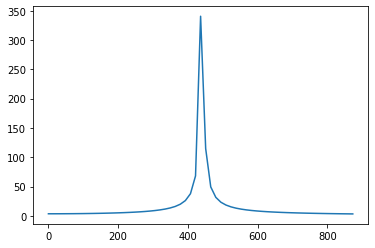
\includegraphics[scale=1]{fig/lab03/lab03_4_0.png}
		\caption{Рассматриваемый сигнал}
	\end{center}
\end{figure}

Посмотрим как выглядит спектограмма с использованием окна Хэмминга:

\begin{figure}[H]
	\begin{center}
		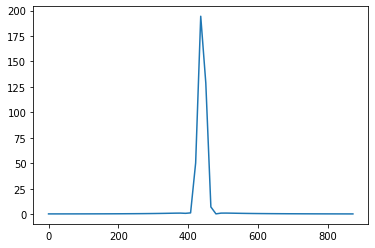
\includegraphics[scale=1]{fig/lab03/lab03_6_0.png}
		\caption{Сигнал с использованием окна Хэмминга}
	\end{center}
\end{figure}

Посмотрим остальные окна


Окно Бартлетта:
\begin{lstlisting}[language=Python]
wave = signal.make_wave(duration)
wave.ys *= np.bartlett(len(wave.ys))
spectrum = wave.make_spectrum()
spectrum.plot(high=880)
\end{lstlisting}
\begin{figure}[H]
	\begin{center}
		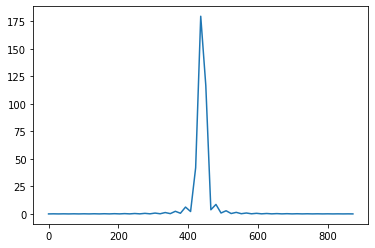
\includegraphics[scale=1]{fig/lab03/lab03_9_0.png}
		\caption{Сигнал с использованием окна Барлетта}
	\end{center}
\end{figure}
Можно заметить. что низкие амплитуды стали ломанными линиями.


Окно Блэкмена:
\begin{lstlisting}[language=Python]
wave = signal.make_wave(duration)
wave.ys *= np.blackman(len(wave.ys))
spectrum = wave.make_spectrum()
spectrum.plot(high=880)
\end{lstlisting}
\begin{figure}[H]
	\begin{center}
		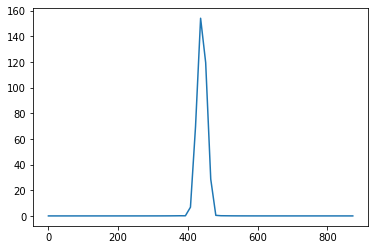
\includegraphics[scale=1]{fig/lab03/lab03_12_0.png}
		\caption{Сигнал с использованием окна Блэкмена}
	\end{center}
\end{figure}

Видим. что утечка стала линейно переходить к нужной частоте.

Окно Хэннинга:
\begin{lstlisting}[language=Python]
wave = signal.make_wave(duration)
wave.ys *= np.hanning(len(wave.ys))
spectrum = wave.make_spectrum()
spectrum.plot(high=880)
\end{lstlisting}
\begin{figure}[H]
	\begin{center}
		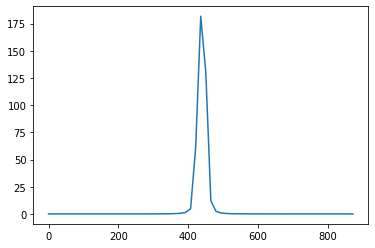
\includegraphics[scale=1]{fig/lab03/lab03_15_0.png}
		\caption{Сигнал с использованием окна Хэннинга}
	\end{center}
\end{figure}

Все оконные функции хорошо справились со своими задачами.
\subsection{Упражнение 2}


Напишите класс SawtoothChirp, расширяющий Chirp и переопределяющий evaluate для генерации пилообразного сигнала с линейно увеличивающейся частотой.

\noindent Нарисуйте эскиз спектограммы этого сигнала, затем распечатайте её. Эффект биение должен быть очевиден, а если сигнал внимательно прослушать, то биения можно и услышать.

\begin{lstlisting}[language=Python]
class SawtoothChirp(Chirp):

    def evaluate(self, ts):
        
        freqs = np.linspace(self.start, self.end, len(ts))
        dts = np.diff(ts, prepend=0)
        dphis = 2 * np.pi * freqs * dts
        phases = np.cumsum(dphis)
        cycles = phases / (2 * np.pi)
        frac, _ = np.modf(cycles)
        ys =  normalize(unbias(frac), self.amp)
        return ys
\end{lstlisting}

Создадим звук:

\begin{lstlisting}[language=Python]
signal = SawtoothChirp(start = 440, end = 880)
wave = signal.make_wave(duration=1, framerate=4000)
wave.make_audio()
\end{lstlisting}

Слышно, как частота постепенно увеливается.

Выполним кратковременное преобразование Фурье и представим результат в виде спектограммы. По оси OY будет частота, по оси OX время.

\begin{lstlisting}[language=Python]
sp = wave.make_spectrogram(256)
sp.plot()
\end{lstlisting}
\begin{figure}[H]
	\begin{center}
		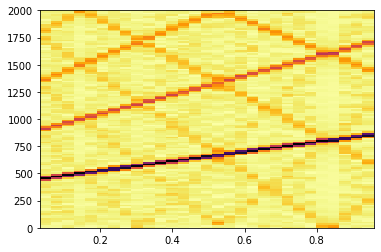
\includegraphics[scale=1]{fig/lab03/lab03_23_0.png}
		\caption{КПФ сигнала}
	\end{center}
\end{figure}

Черной линией обозначена наша основная частота, остальные частоты "отпрыгивают" от рамок координат и слышны на заднем плане.

\subsection{Упражнение 3}

Создайте пилообразный чирп, меняющийся от 2500 до 3000 Гц, и на его основе сгенерируйте сигнал длительностью 1 с и частотой кадоров 20 кГц. Нарисуйте, каким примерно будет Spectrum. Затем распечатайте Spectrum и посмотрите, правы ли вы.

\begin{lstlisting}[language=Python]
signal = SawtoothChirp(start=2500, end=3000)
wave = signal.make_wave(duration=1, framerate=20000)

wave.make_spectrum().plot()
\end{lstlisting}
\begin{figure}[H]
	\begin{center}
		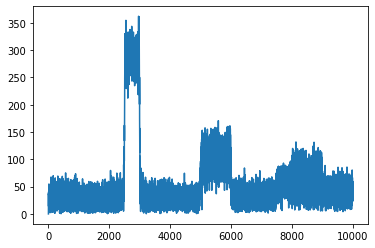
\includegraphics[scale=1]{fig/lab03/lab03_27_0.png}
		\caption{Спектр сигнала}
	\end{center}
\end{figure}

Видим, что гармоники накладываются друг на друга, и заметно что на частоте 2500 появляется возвышенность и на частоте около 5000 тоже. Это связано с тем, что в данном диапозоне равное изменение частоты занимает равное время.

\subsection{Упражнение 4}

В музыкальной терминологии «глиссандо» — это нота, которая скользит от одной высоты тона к другой, поэтому она похожа на чириканье. Найдите или сделайте запись глиссандо и постройте его спектрограмму.

Возьмём звук из репозитория учебника:

\begin{lstlisting}[language=Python]
if not os.path.exists('72475__rockwehrmann__glissup02.wav'):
    !wget https://github.com/AllenDowney/ThinkDSP/raw/master/code/72475__rockwehrmann__glissup02.wav
    

wave = read_wave('72475__rockwehrmann__glissup02.wav')

wave.make_spectrogram(512).plot(high=5000)
\end{lstlisting}
\begin{figure}[H]
	\begin{center}
		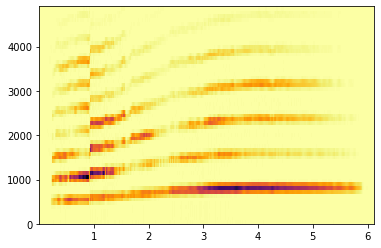
\includegraphics[scale=1]{fig/lab03/lab03_32_0.png}
		\caption{Спектрограмма сигнала}
	\end{center}
\end{figure}

Видим, что спектограмма очень похожа на наш чирп.

\subsection{Упражнение 5}

Тромбонист может играть глиссандо, выдвигая слайд тромбона и непрерывно дуя. По мере выдвижения ползуна общая длина трубки увеличивается, а результирующий шаг обратно пропорционален длине.
Предполагая, что игрок перемещает слайд с постоянной скоростью, как меняется ли частота со временем?

\noindent Напишите класс TromboneGliss, расширяющий класс Chirp и предоставляет evaluate. Создайте волну, имитирующую тромбон глиссандо от F3 вниз до C3 и обратно до F3. C3 — 262 Гц; F3 есть 349 Гц.

\begin{lstlisting}[language=Python]
class TromboneGliss(Chirp):

    
    def evaluate(self, ts):
        lengths = np.linspace(1.0 / self.start, 1.0 / self.end, len(ts))
        freqs = 1 / lengths
        dts = np.diff(ts, prepend=0)
        dphis = np.pi * 2 * freqs * dts
        phases = np.cumsum(dphis)
        ys = self.amp * np.cos(phases)
        return ys
\end{lstlisting}

Соединим сигналы:
\begin{lstlisting}[language=Python]
signal1 = TromboneGliss(262, 349)
wave1 = signal.make_wave(duration=1)

signal2 = TromboneGliss(349, 262)
wave2 = signal2.make_wave(duration=1)

result = wave1 | wave2
sp = result.make_spectrogram(1024)
sp.plot(high=1000)
\end{lstlisting}
\begin{figure}[H]
	\begin{center}
		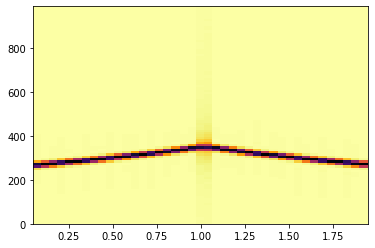
\includegraphics[scale=1]{fig/lab03/lab03_42_0.png}
		\caption{Спектрограмма сигнала}
	\end{center}
\end{figure}

Отчётливо слышно, как идут друг за другом 2 части.


\subsection{Упражнение 6}

Сделайте или найдите запись серии гласных звуков и посмотрите на спектрограмму. Сможете ли вы различить разные гласные?

Возьмём гласные из репозитория учебника:

\begin{lstlisting}[language=Python]
if not os.path.exists('87778__marcgascon7__vocals.wav'):
    !wget https://github.com/AllenDowney/ThinkDSP/raw/master/code/87778__marcgascon7__vocals.wav
wave = read_wave('87778__marcgascon7__vocals.wav')
wave.make_spectrogram(1024).plot(1000)
\end{lstlisting}
\begin{figure}[H]
	\begin{center}
		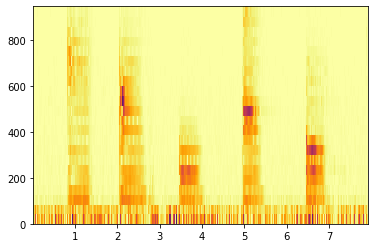
\includegraphics[scale=1]{fig/lab03/lab03_47_0.png}
		\caption{Спектрограмма гласных звуков}
	\end{center}
\end{figure}

На спектограмме видны пики, они и будут нашими гласными.

\subsection{Вывод}

В этой работе были расмотрены апериодические сигналы, частотные компоненты которых изменяются во времени. Также в этой главе были рассмотрены спектрограммы - способ визуализации апериодичных сигналов.
\newpage

\section{Шумы}
\subsection{Упражнение 1}

«A Soft Murmur» — это веб-сайт, на котором можно послушать множество естественных источников шума, включая дождь, волны, ветер и т. д. 

\noindent На http://asoftmurmur.com/about/ вы можете найти их список записей, большинство из которых находится на http://freesound.org.

\noindent Загрузите несколько таких файлов и вычислите спектр каждого сигнала. Спектр мощности похож на белый шум, розовый шум, или броуновский шум? Как изменяется спектр во времени?

Возьмём звук свёрчков и вырежем сегемент. Мне кажется шум будет скоррелирован.

\begin{lstlisting}[language=Python]
wave = read_wave('22604__martypinso__dmp010037-crickets-texas.wav')
segment = wave.segment(start=10, duration=1.0)
segment.plot()
\end{lstlisting}
\begin{figure}[H]
	\begin{center}
		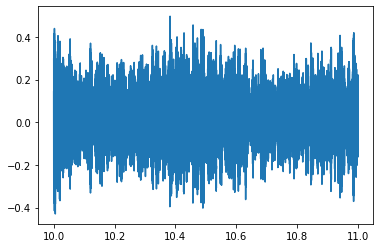
\includegraphics[scale=1]{fig/lab04/lab04_7_0.png}
		\caption{График сигнала}
	\end{center}
\end{figure}

Для определения характеристик шума используем код из пособия по построению графика спекта в логорифмическом масштабе.

\begin{lstlisting}[language=Python]
from thinkdsp import decorate
spectrum.plot_power()

loglog = dict(xscale='log', yscale='log')
decorate(xlabel='Frequency (Hz)',
         ylabel='Power', 
         **loglog)
\end{lstlisting}
\begin{figure}[H]
	\begin{center}
		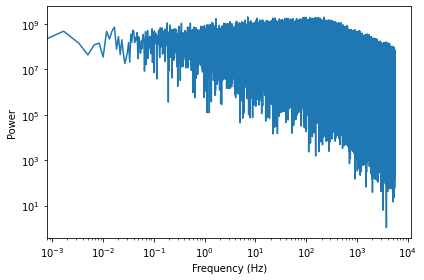
\includegraphics[scale=1]{fig/lab04/lab04_9_0.png}
		\caption{Спектр в логорифмическом масштабе}
	\end{center}
\end{figure}

Давайте возьмём следующий сегмент для наглядности.

\begin{lstlisting}[language=Python]
segment1 = wave.segment(start=11, duration=1.0)
spectrum1 = segment1.make_spectrum()
spectrum.plot_power()
spectrum1.plot_power()


loglog = dict(xscale='log', yscale='log')
decorate(xlabel='Frequency (Hz)',
         ylabel='Power', 
         **loglog)
\end{lstlisting}
\begin{figure}[H]
	\begin{center}
		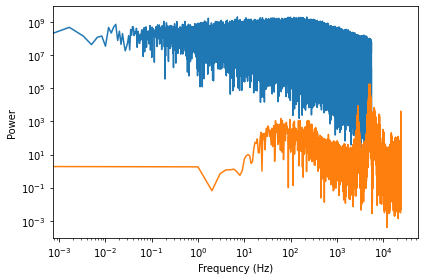
\includegraphics[scale=1]{fig/lab04/lab04_12_0.png}
		\caption{Сравнение спектров в логорифмическом масштабе}
	\end{center}
\end{figure}

\begin{lstlisting}[language=Python]
noise = UncorrelatedGaussianNoise()
wave2 = noise.make_wave(duration=1)
spectrum2 = wave2.make_spectrum()
spectrum.plot_power()
spectrum2.plot_power()


loglog = dict(xscale='log', yscale='log')
decorate(xlabel='Frequency (Hz)',
         ylabel='Power', 
         **loglog)
\end{lstlisting}

Оранжевым обозначен Гауссов шум.

\begin{figure}[H]
	\begin{center}
		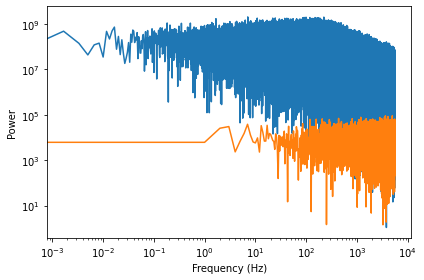
\includegraphics[scale=1]{fig/lab04/lab04_14_0.png}
		\caption{Сравнение нашего звука с Гауссовым шумом}
	\end{center}
\end{figure}

\subsection{Упражнение 2}

Реализуйте метод Бартлетта\cite{barlett} и используйте его для оценки спектра мощности шумового сигнала. Подсказка: посмотрите на реализацую make\_spectrogram.

Исходя из статьи на википедии надо поделить данные на сегменты, потом для каждого сегмента сделать разложение Фурье, вычислить сумму квадратов и раздлелить на количество элементов и взять от этого всего корень.

Посмотрим с помощью чего и как создаются спектограммы:

\begin{lstlisting}[language=Python]
    def make_spectrogram(self, seg_length, win_flag=True):
        """Computes the spectrogram of the wave.
        seg_length: number of samples in each segment
        win_flag: boolean, whether to apply hamming window to each segment
        returns: Spectrogram
        """
        if win_flag:
            window = np.hamming(seg_length)
        i, j = 0, seg_length
        step = int(seg_length // 2)

        # map from time to Spectrum
        spec_map = {}

        while j < len(self.ys):
            segment = self.slice(i, j)
            if win_flag:
                segment.window(window)

            # the nominal time for this segment is the midpoint
            t = (segment.start + segment.end) / 2
            spec_map[t] = segment.make_spectrum()

            i += step
            j += step

        return Spectrogram(spec_map, seg_length)
\end{lstlisting}
\begin{lstlisting}[language=Python]
        """Initializes a spectrum.
        hs: array of amplitudes (real or complex)
        fs: array of frequencies
        framerate: frames per second
        full: boolean to indicate full or real FFT
        """
        self.hs = np.asanyarray(hs)
        self.fs = np.asanyarray(fs)
        self.framerate = framerate
        self.full = full
\end{lstlisting}

Для создания своей функции надо изменять словарь:
\begin{lstlisting}[language=Python]
def make_barlett(wave, N, flag=True):
  spectrogram = wave.make_spectrogram(N,flag)
  spec_mac = spectrogram.spec_map.values()

  powers = []
  for spectrum in spec_mac:
    powers.append(spectrum.power)
  
  hs = np.sqrt(sum(powers)/ len(powers))
  fs = next(iter(spec_mac)).fs

  return Spectrum(hs, fs, wave.framerate)
\end{lstlisting}

\begin{lstlisting}[language=Python]
barlett = make_barlett(segment,1024)
barlett.plot_power()

decorate(xlabel='Frequency (Hz)', 
         ylabel='Power', 
         **loglog)
\end{lstlisting}
\begin{figure}[H]
	\begin{center}
		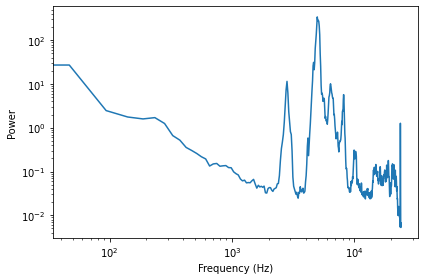
\includegraphics[scale=1]{fig/lab04/lab04_23_0.png}
		\caption{Результат}
	\end{center}
\end{figure}


\subsection{Упражнение 3}

Загрузите в виде CSV-файла исторические данные о ежедневной цене BitCoin. Откройте этот файл и вычислите спектр цен BitCoin как функцию времени. Похоже ли это на белый, розовый или броуновский шум?

\begin{lstlisting}[language=Python]
  if not os.path.exists('market-price.csv'):
    !wget https://github.com/wooftown/spbstu-telecom/raw/main/Content/market-price.csv
\end{lstlisting}
\begin{lstlisting}[language=Python]
import csv

worth = []

with open('market-price.csv') as File:
  reader = csv.reader(File, delimiter=',', quotechar=',',
                        quoting=csv.QUOTE_MINIMAL)
  worth = [row[1] for row in reader]

worth = worth [1:]
days = a=np.arange(0,len(worth))
\end{lstlisting}
\begin{lstlisting}[language=Python]
wave = Wave(worth,days,1)
wave.plot()
decorate(xlabel='Time (days)')
\end{lstlisting}
\begin{figure}[H]
	\begin{center}
		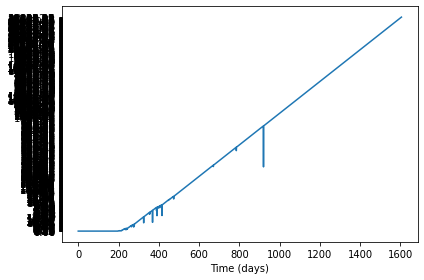
\includegraphics[scale=1]{fig/lab04/lab04_28_0.png}
		\caption{График цен BitCoin}
	\end{center}
\end{figure}

График получился не очень красивым из-за того, что слишком много данных, можно приблизить и посмотреть какой-то один сегмент. Давайте перейдём к спектограмме.

\begin{lstlisting}[language=Python]
spectrum = wave.make_spectrum()
spectrum.plot_power()
decorate(xlabel='Frequency (1/days)',
         ylabel='Power', 
         **loglog)
\end{lstlisting}
\begin{figure}[H]
	\begin{center}
		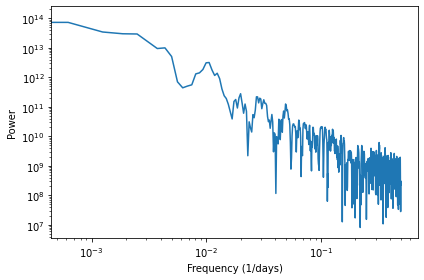
\includegraphics[scale=1]{fig/lab04/lab04_32_0.png}
		\caption{Спектрограмма цен BitCoin в логорифмическом формате}
	\end{center}
\end{figure}

Больше всего это походе на красный шум, так как связь похожа на отбраную квадратную.

\subsection{Упражнение 4}

Счетчик Гейгера — это прибор, который регистрирует радиацию. Когда ионизирующая частица попадает на детектор, он генерирует всплеск тока. Общий вывод в определенный момент времени можно смоделировать как некоррелированный шум Пуассона (UP), где каждая выборка представляет собой случайную величину из распределения Пуассона, которая соответствует количеству частиц, обнаруженных в течение интервала.

Напишите класс с именем `UncorrelatedPoissonNoise`, который наследуется от `\_Noise` и предоставляет `evaluate`. Он должен использовать `np.random.poisson` для генерации случайных значений из распределения Пуассона. Параметр этой функции, lam, представляет собой среднее число частиц в течение каждого интервала. Вы можете использовать атрибут `amp`, чтобы указать `lam`. Например, если частота кадров равна 10 кГц, а amp равно 0,001, мы ожидаем около 10 «кликов» в секунду.

Создайте около секунды шума UP и послушайте его. Для низких значений «ампер», например 0,001, это должно звучать как счетчик Гейгера. Для более высоких значений это должно звучать как белый шум. Вычислите и начертите спектр мощности, чтобы увидеть, похож ли он на белый шум.

\begin{lstlisting}[language=Python]
class UncorrelatedPoissonNoise(Noise):
  def evaluate(self, ts):
    ys = np.random.poisson(self.amp,len(ts))
    return ys
\end{lstlisting}
\begin{lstlisting}[language=Python]
noise1 = UncorrelatedPoissonNoise(0.001)
wave1 = noise1.make_wave(duration=1,framerate = 11025)
wave1.plot()
\end{lstlisting}
\begin{figure}[H]
	\begin{center}
		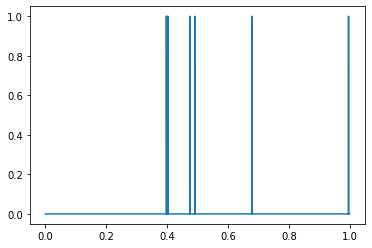
\includegraphics[scale=1]{fig/lab04/lab04_37_0.png}
		\caption{Получившийся сигнал}
	\end{center}
\end{figure}

\begin{lstlisting}[language=Python]
noise2 = UncorrelatedPoissonNoise(1)
wave2 = noise2.make_wave(duration=1,framerate = 11025)
wave2.plot()
\end{lstlisting}
\begin{figure}[H]
	\begin{center}
		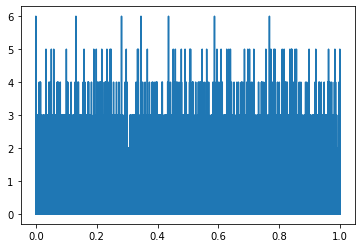
\includegraphics[scale=1]{fig/lab04/lab04_39_0.png}
		\caption{Получившийся сигнал}
	\end{center}
\end{figure}
\begin{lstlisting}[language=Python]
spectrum1 = wave1.make_spectrum()
spectrum2 = wave2.make_spectrum()
spectrum1.plot_power()
spectrum2.plot_power()

decorate(xlabel='Frequency (Hz)', 
         ylabel='Power', 
         **loglog)
\end{lstlisting}
\begin{figure}[H]
	\begin{center}
		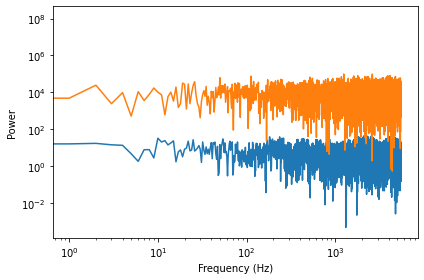
\includegraphics[scale=1]{fig/lab04/lab04_41_0.png}
		\caption{Сравнение спектров}
	\end{center}
\end{figure}

При увеличении значения ампилутуды сигнал всё больше походит на белый шум.
\subsection{Упражнение 5}

В этой главе описан алгоритм генерации розового шума. Концептуально простой, но вычислительно затратный. Есть более эффективные альтернативы, такие как алгоритм Восса-Маккартни.

\noindent Исследуйте этот метод, реализуйте его, вычислите спектр и подтвердите, что он имеет желаемое отношение между мощностью и частотой.

\begin{lstlisting}[language=Python]
def iterpink(depth):
    values = np.random.randn(depth)
    smooth = np.random.randn(depth)
    source = np.random.randn(depth)
    sumvals = values.sum()
    i = 0
    while True:
        yield sumvals + smooth[i]
        i += 1
        if i == depth:
            i = 0
            smooth = np.random.randn(depth)
            source = np.random.randn(depth)
            continue
        c = 0
        while not (i >> c) & 1:
            c += 1
        sumvals += source[i] - values[c]
        values[c] = source[i]
\end{lstlisting}

\begin{lstlisting}[language=Python]
def pink_noise(points, depth=16):
    a = []
    s = iterpink(depth)
    for n in range(points):
        a.append(next(s))
    return np.array(a)
\end{lstlisting}

\begin{lstlisting}[language=Python]
ys = pink_noise(11025,16)
wave = Wave(ys)
wave.plot()
\end{lstlisting}
\begin{figure}[H]
	\begin{center}
		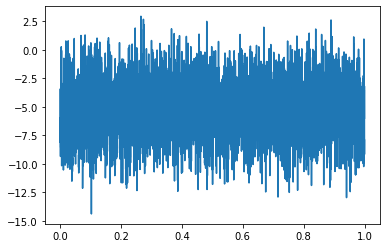
\includegraphics[scale=1]{fig/lab04/lab04_47_0.png}
		\caption{Сгенерированный сигнал}
	\end{center}
\end{figure}

В итоге получили сигнал розового шума:
\begin{lstlisting}[language=Python]
spectrum = wave.make_spectrum()
spectrum.hs[0] = 0
spectrum.plot_power()
decorate(xlabel='Frequency (Hz)',
         ylabel='Power',
         **loglog)
\end{lstlisting}
\begin{figure}[H]
	\begin{center}
		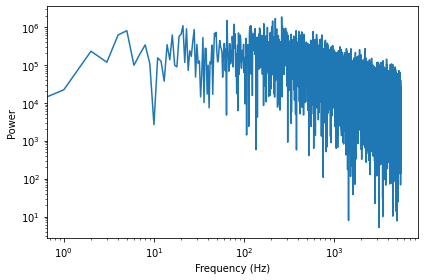
\includegraphics[scale=1]{fig/lab04/lab04_50_0.png}
		\caption{Розовый шум}
	\end{center}
\end{figure}

\subsection{Вывод}

В этой работе был рассмотрен шум. Шум - сигнал, содержащий компоненты с самыми разными частотами, но не имеющий гармонической структуры периодических сигналов, рассмотреных в предыдущих работах.
\newpage

\section{Автокорреляция }
\subsection{Упражнение 1}

Оцените высоты тона вокального чирпа для нескольких времён начала сегмента.

\begin{lstlisting}[language=Python]
if not os.path.exists('28042__bcjordan__voicedownbew.wav'):
    !wget https://github.com/AllenDowney/ThinkDSP/raw/master/code/28042__bcjordan__voicedownbew.wav
wave = read_wave('code_28042__bcjordan__voicedownbew.wav')
wave.normalize()
duration = 0.01
segment1 = wave.segment(start=0.1, duration=duration)
segment1.plot()
segment2 = wave.segment(start=0.2, duration=duration)
segment2.plot()
segment3 = wave.segment(start=0.3, duration=duration)
segment3.plot()
\end{lstlisting}
\begin{figure}[H]
	\begin{center}
		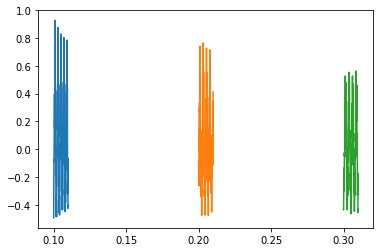
\includegraphics[scale=1]{fig/lab05/lab05_5_0.png}
		\caption{График выбранных сегментов}
	\end{center}
\end{figure}

Для определения высоты тона используем автокореляцию.

\begin{lstlisting}[language=Python]
lags1, corrs1 = autocorr(segment1)
plt.plot(lags1, corrs1, color='green')
decorate(xlabel='Lag (index)', ylabel='Correlation', ylim=[-1, 1])

lags2, corrs2 = autocorr(segment2)
plt.plot(lags2, corrs2)
decorate(xlabel='Lag (index)', ylabel='Correlation', ylim=[-1, 1])

lags3, corrs3 = autocorr(segment3)
plt.plot(lags3, corrs3, color='red')
decorate(xlabel='Lag (index)', ylabel='Correlation', ylim=[-1, 1])
\end{lstlisting}
\begin{figure}[H]
	\begin{center}
		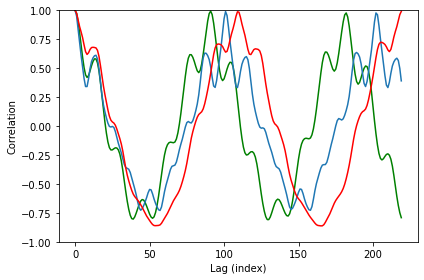
\includegraphics[scale=1]{fig/lab05/lab05_7_0.png}
		\caption{Автокорреляция сигналов}
	\end{center}
\end{figure}

Узнаем значения lag:

\begin{lstlisting}[language=Python]
low, high = 50, 200
lag1 = np.array(corrs1[low:high]).argmax() + low

low, high = 50, 200
lag2 = np.array(corrs2[low:high]).argmax() + low

low, high = 50, 200
lag3 = np.array(corrs3[low:high]).argmax() + low

lag1,lag2, lag3
\end{lstlisting}
\begin{lstlisting}
(91, 101, 109)
\end{lstlisting}

Периоды:

\begin{lstlisting}[language=Python]
period1 = lag1 / segment1.framerate
period2 = lag2 / segment2.framerate
period3 = lag3 / segment3.framerate
period1, period2, period3
\end{lstlisting}
\begin{lstlisting}
(0.0020634920634920637, 0.002290249433106576, 0.002471655328798186)
\end{lstlisting}

F max:

\begin{lstlisting}[language=Python]
frequency1 = 1 / period1
frequency2 = 1 / period2
frequency3 = 1 / period3
frequency1, frequency2, frequency3
\end{lstlisting}
\begin{lstlisting}
(484.6153846153846, 436.63366336633663, 404.5871559633028)
\end{lstlisting}

\subsection{Упражнение 2}
Инкапсулировать код автокорреляции для оценки основной частоты периодического сигнала в функцию, названную estimate\_fundamental, и исользуйте её для отслеживания высоты тона записанного звука.

Возьмём тот же звук.

\begin{lstlisting}[language=Python]
wave.make_spectrogram(2048).plot(high=4000)
\end{lstlisting}
\begin{figure}[H]
	\begin{center}
		\includegraphics[scale=1]{fig/lab05/lab05_16_0.png}
		\caption{Спектрограмма записи}
	\end{center}
\end{figure}

Берём код из предыдущих пунктов и соединияем в одну функцию:

\begin{lstlisting}[language=Python]
def estimate_fundamental(segment, low=50, high=200):
  lags, corrs = autocorr(segment)
  lag = np.array(corrs[low:high]).argmax() + low
  period = lag / segment.framerate
  frequency = 1 / period
  return frequency
\end{lstlisting}

\begin{lstlisting}[language=Python]
estimate_fundamental(segment1)
\end{lstlisting}
\begin{lstlisting}
484.6153846153846
\end{lstlisting}

Чтобы сделать оценку высоты тона на всей спектрограмме надо разделить всё на маленькие сегменты и работать с ними.

\begin{lstlisting}[language=Python]
duration = wave.duration
step = 0.02
start = 0
time = []
freq = []
while start + step < duration:
  time.append(start + step/2)
  freq.append(estimate_fundamental(wave.segment(start=start,duration=step)))
  start += step
wave.make_spectrogram(2048).plot(high=900)
plt.plot(time, freq, color='blue')
decorate(xlabel='Time (s)', ylabel='Frequency (Hz)')
\end{lstlisting}
\begin{figure}[H]
	\begin{center}
		\includegraphics[scale=1]{fig/lab05/lab05_22_0.png}
		\caption{Результат}
	\end{center}
\end{figure}

\subsection{Упражнение 3}

Вычислить автокорреляцию цен в платёжной системе Bitcoin. Оценить автокореляцию и проверить на признаки переодичности процесса.

\begin{lstlisting}[language=Python]
if not os.path.exists('market-price.csv'):
    !wget https://github.com/wooftown/spbstu-telecom/raw/main/Content/market-price.csv
import pandas as pd

df = pd.read_csv('market-price.csv', parse_dates=[0])
ys = df['market-price']
ts = df.index

w = Wave(ys, framerate=1)
w.plot()

\end{lstlisting}
\begin{figure}[H]
	\begin{center}
		\includegraphics[scale=1]{fig/lab05/lab05_25_0.png}
		\caption{График цены на BitCoin}
	\end{center}
\end{figure}

Вычислим автокорреляцию:

\begin{lstlisting}[language=Python]
lags, corrs = autocorr(w)
plt.plot(lags, corrs)
decorate(xlabel='Lag',
         ylabel='Correlation')
\end{lstlisting}
\begin{figure}[H]
	\begin{center}
		\includegraphics[scale=1]{fig/lab05/lab05_27_0.png}
		\caption{Автокорреляция функции цены на BitCoin}
	\end{center}
\end{figure}

Функция ведёт себя нестабильно, есть резкие повышения и спады. Имеется намёк на периодичность.

\subsection{Упражнение 4}

В репозитории этой книги есть блокнот Jupyter под названием saxophone.ipynb, в котором исследуются автокорреляция, восприятие высоты тона и явление, называемое подавленная основная. Прочтите этот блокнот и «погоняйте» примеры. Выберите другой сегмент записи и вновь поработайте с примерами.

\begin{lstlisting}[language=Python]
if not os.path.exists('100475__iluppai__saxophone-weep.wav'):
    !wget https://github.com/AllenDowney/ThinkDSP/raw/master/code/100475__iluppai__saxophone-weep.wav
wave = read_wave('100475__iluppai__saxophone-weep.wav')
wave.normalize()
spectrogram = wave.make_spectrogram(seg_length=1024)
spectrogram.plot(high=3000)
decorate(xlabel='Time (s)', ylabel='Frequency (Hz)')
\end{lstlisting}
\begin{figure}[H]
	\begin{center}
		\includegraphics[scale=1]{fig/lab05/lab05_33_0.png}
		\caption{Спектрограмма звука}
	\end{center}
\end{figure}

Видна гармоническая структура во времени. Возьмём отрезок и прогоним его через все функции из блокнота.

\begin{lstlisting}[language=Python]
segment = wave.segment(start=1, duration=0.2)
segment.make_audio()
\end{lstlisting}

\begin{lstlisting}[language=Python]
spectrum = segment.make_spectrum()
spectrum.plot(high=5000)
decorate(xlabel='Frequency (Hz)', ylabel='Amplitude')
\end{lstlisting}
\begin{figure}[H]
	\begin{center}
		\includegraphics[scale=1]{fig/lab05/lab05_37_0.png}
		\caption{Спектр звука}
	\end{center}
\end{figure}

Спектр напомнил квадратный сигнал. Пики пришлись на 1245, 415, 830 Гц.

Далее сравним наш сегмент с треугольным сигналом с такой же низкой частотой пика.

\begin{lstlisting}[language=Python]
TriangleSignal(freq=415).make_wave(duration=0.2).make_audio()
\end{lstlisting}

У данных сигналов одинаковая воспринимаемая частота звука.

Для понимания процесса восприятия основной частоты испольщуем АКФ.

\begin{lstlisting}[language=Python]
def autocorr2(segment):
    corrs = np.correlate(segment.ys, segment.ys, mode='same')
    N = len(corrs)
    lengths = range(N, N//2, -1)

    half = corrs[N//2:].copy()
    half /= lengths
    half /= half[0]
    return half
\end{lstlisting}

\begin{lstlisting}[language=Python]
corrs = autocorr2(segment)
plt.plot(corrs[:500])
\end{lstlisting}
\begin{figure}[H]
	\begin{center}
		\includegraphics[scale=1]{fig/lab05/lab05_46_1.png}
		\caption{Автокорреляция}
	\end{center}
\end{figure}

Видим пик рядом с lag 100. Найдём основную частоту при помощи написанной ранее функции.

\begin{lstlisting}[language=Python]
estimate_fundamental(segment)
\end{lstlisting}

Даже если мы уберём основной тон (416 Гц), звук будет восприниматься также...

\begin{lstlisting}[language=Python]
spectrum2 = segment.make_spectrum()
spectrum2.high_pass(600)
spectrum2.plot(high=5000)
decorate(xlabel='Frequency (Hz)', ylabel='Amplitude')
\end{lstlisting}
\begin{figure}[H]
	\begin{center}
		\includegraphics[scale=1]{fig/lab05/lab05_51_0.png}
		\caption{Спектр сигнала}
	\end{center}
\end{figure}

Это явление называется "missing fundamental". Для понимания, что мы слышим частоту которой нет можно снова обратиться к АКФ.

\begin{lstlisting}[language=Python]
corrs = autocorr2(segment2)
plt.plot(corrs[:500])
\end{lstlisting}
\begin{figure}[H]
	\begin{center}
		\includegraphics[scale=1]{fig/lab05/lab05_54_1.png}
		\caption{Автокорреляция}
	\end{center}
\end{figure}


Это так работает, потому что более высокие компоненты сигнала являются гармониками 416 Гц. Весь этот пример указывает нам на то, что восприятие высоты тона основано не только на спектральном анализе, но и на вычислении АКФ.

\subsection{Вывод}

В данной главе была изучена корреляция и её роль в сигналах. Также на пратике был обработан сигнал с "missing fundamental". Когда мы убирали основной тон, всё равно звук звучал также.


\newpage

\section{Дискретное косинусное преобразование }
\subsection{Упражнение 1}

Показать на графике время работы analyze1 и analyze2 в логорифмическом масштабе. Сравнить с scipy.fftpack.dct.

\begin{lstlisting}[language=Python]
def analyze1(ys, fs, ts):
    args = np.outer(ts, fs)
    M = np.cos(PI2 * args)
    amps = np.linalg.solve(M, ys)
    return amps
def analyze2(ys, fs, ts):
    args = np.outer(ts, fs)
    M = np.cos(PI2 * args)
    amps = M.dot(ys) / 2
    return amps
\end{lstlisting}

Возьмём размеры массива как степени 2.

\begin{lstlisting}[language=Python]
ns = 2 ** np.arange(5,10)
\end{lstlisting}

\begin{lstlisting}[language=Python]
best_analyze1 = []
for n in ns:
    ts = (0.5 + np.arange(n)) / n
    freqs = (0.5 + np.arange(n)) / 2
    ys = wave.ys[:n]
    best =  %timeit -r1 -o analyze1(ys,freqs,ts)
    best_analyze1.append(best.best)
best_analyze2 = []
for n in ns:
    ts = (0.5 + np.arange(n)) / n
    freqs = (0.5 + np.arange(n)) / 2
    ys = wave.ys[:n]
    best =  %timeit -r1 -o analyze2(ys,freqs,ts)
    best_analyze2.append(best.best)
best_dct = []
for n in ns:
    ys = wave.ys[:n]
    best =  %timeit -r1 -o scipy.fftpack.dct(ys, type=3)
    best_dct.append(best.best)
plt.plot(ns, best_analyze1, label='analyze1')
plt.plot(ns, best_analyze2, label='analyze2')
plt.plot(ns, best_dct, label='fftpack.dct')
loglog = dict(xscale='log', yscale='log')
decorate(xlabel='Wave length (N)', ylabel='Time (s)', **loglog)
\end{lstlisting}

\begin{figure}[H]
	\begin{center}
		\includegraphics[scale=1]{fig/lab06/lab06_18_0.png}
		\caption{Время работы различных методов ДКП}
	\end{center}
\end{figure}

Не смотря на теоритическое время исполнения, время analyze1 получилсось пропорциональным  n2 .

\subsection{Упражнение 2}

Реализовать алгоритм сжатия для музыки или речи.

Выберем звук для сжатия:
\begin{lstlisting}[language=Python]
if not os.path.exists('164718__bradovic__piano.wav'):
    !wget https://github.com/wooftown/spbstu-telecom/raw/main/Content/164718__bradovic__piano.wav
    wave = read_wave('164718__bradovic__piano.wav')
\end{lstlisting}

Для начала возьмём небольшой сегмент:

\begin{lstlisting}[language=Python]
segment = wave.segment(start = 1.7,duration = 1.0)
segment.normalize()
segment.make_audio()
\end{lstlisting}

Вместо DFT используем DCT.

\begin{lstlisting}[language=Python]
dct = segment.make_dct()
dct.plot(high = 5000)
\end{lstlisting}
\begin{figure}[H]
	\begin{center}
		\includegraphics[scale=1]{fig/lab06/lab06_29_0.png}
		\caption{Спектр сигнала полученный при помощи ДКП}
	\end{center}
\end{figure}

\begin{lstlisting}[language=Python]
def filtering(dct,limit = 0):
  for i, amp in enumerate(dct.amps):
    if np.abs(amp) < limit:
      dct.hs[i] = 0
\end{lstlisting}

\begin{lstlisting}[language=Python]
filtering(dct,1000)
dct.plot(high = 5000)
\end{lstlisting}
\begin{figure}[H]
	\begin{center}
		\includegraphics[scale=1]{fig/lab06/lab06_32_0.png}
		\caption{ДКП после фильтрации}
	\end{center}
\end{figure}

Теперь осталось подобрать значение, чтобы выходной файл звучал как входной. Для сохранения памяти необходимо использовать разряженные массивы.

\subsection{Управжнение 3}

В блокноте phase.ipynb взять другой сегмент звука и повторить эксперименты.

\begin{lstlisting}[language=Python]
signal = SawtoothSignal(freq=500, offset=0)
wave = signal.make_wave(duration=0.5, framerate=40000)
wave.segment(start=0.005,duration=0.01).plot()
decorate(xlabel='Time (s)')
\end{lstlisting}
\begin{figure}[H]
	\begin{center}
		\includegraphics[scale=1]{fig/lab06/lab06_41_0.png}
		\caption{Выбранный сегмент}
	\end{center}
\end{figure}

\begin{lstlisting}[language=Python]
spectrum = wave.make_spectrum()
spectrum.plot()
decorate(xlabel='Frequency (Hz)',
         ylabel='Amplitude')
\end{lstlisting}
\begin{figure}[H]
	\begin{center}
		\includegraphics[scale=1]{fig/lab06/lab06_42_0.png}
		\caption{Спектр сегемента}
	\end{center}
\end{figure}

\begin{lstlisting}[language=Python]
def plot_angle(spectrum, thresh=1):
    angles = spectrum.angles
    angles[spectrum.amps < thresh] = np.nan
    plt.plot(spectrum.fs, angles, 'x')
    decorate(xlabel='Frequency (Hz)', 
             ylabel='Phase (radian)')
             
def plot_three(spectrum, thresh=1):
    """Plot amplitude, phase, and waveform.
    
    spectrum: Spectrum object
    thresh: threshold passed to plot_angle
    """
    plt.figure(figsize=(10, 4))
    plt.subplot(1,3,1)
    spectrum.plot()
    plt.subplot(1,3,2)
    plot_angle(spectrum, thresh=thresh)
    plt.subplot(1,3,3)
    wave = spectrum.make_wave()
    wave.unbias()
    wave.normalize()
    wave.segment(duration=0.01).plot()
    display(wave.make_audio())

def zero_angle(spectrum):
    res = spectrum.copy()
    res.hs = res.amps
    return res
    
def rotate_angle(spectrum, offset):
    res = spectrum.copy()
    res.hs *= np.exp(1j * offset)
    return res

def random_angle(spectrum):
    res = spectrum.copy()
    angles = np.random.uniform(0, PI2, len(spectrum))
    res.hs *= np.exp(1j * angles)
    return res
\end{lstlisting}

\begin{lstlisting}[language=Python]
plot_three(spectrum)
\end{lstlisting}
\begin{figure}[H]
	\begin{center}
		\includegraphics[scale=0.66]{fig/lab06/lab06_47_1.png}
		\caption{Получившиеся графики}
	\end{center}
\end{figure}

\begin{lstlisting}[language=Python]
spectrum2 = zero_angle(spectrum)
plot_three(spectrum2)
\end{lstlisting}
\begin{figure}[H]
	\begin{center}
		\includegraphics[scale=0.66]{fig/lab06/lab06_49_1.png}
		\caption{Получившиеся графики}
	\end{center}
\end{figure}


\begin{lstlisting}[language=Python]
spectrum3 = rotate_angle(spectrum, 1)
plot_three(spectrum3)
\end{lstlisting}
\begin{figure}[H]
	\begin{center}
		\includegraphics[scale=0.66]{fig/lab06/lab06_51_1.png}
		\caption{Получившиеся графики}
	\end{center}
\end{figure}


\begin{lstlisting}[language=Python]
spectrum4 = random_angle(spectrum)
plot_three(spectrum4)
\end{lstlisting}
\begin{figure}[H]
	\begin{center}
		\includegraphics[scale=0.66]{fig/lab06/lab06_54_1.png}
		\caption{Получившиеся графики}
	\end{center}
\end{figure}

Теперь возьмём другой звук и сделаем всё тоже самое:

\begin{lstlisting}[language=Python]
if not os.path.exists('120994__thirsk__120-oboe.wav'):
    !wget https://github.com/AllenDowney/ThinkDSP/raw/master/code/120994__thirsk__120-oboe.wav
wave = read_wave('120994__thirsk__120-oboe.wav')
segment = wave.segment(start=0.1, duration=0.5)
spectrum = segment.make_spectrum()
\end{lstlisting}

\begin{lstlisting}[language=Python]
plot_three(spectrum)
\end{lstlisting}
\begin{figure}[H]
	\begin{center}
		\includegraphics[scale=0.66]{fig/lab06/lab06_58_1.png}
		\caption{Получившиеся графики}
	\end{center}
\end{figure}

\begin{lstlisting}[language=Python]
spectrum2 = zero_angle(spectrum)
plot_three(spectrum2)
\end{lstlisting}
\begin{figure}[H]
	\begin{center}
		\includegraphics[scale=0.66]{fig/lab06/lab06_59_1.png}
		\caption{Получившиеся графики}
	\end{center}
\end{figure}


\begin{lstlisting}[language=Python]
spectrum3 = rotate_angle(spectrum, 1)
plot_three(spectrum3)
\end{lstlisting}
\begin{figure}[H]
	\begin{center}
		\includegraphics[scale=0.66]{fig/lab06/lab06_61_1.png}
		\caption{Получившиеся графики}
	\end{center}
\end{figure}


\begin{lstlisting}[language=Python]
spectrum4 = random_angle(spectrum)
plot_three(spectrum4)
\end{lstlisting}
\begin{figure}[H]
	\begin{center}
		\includegraphics[scale=0.66]{fig/lab06/lab06_63_1.png}
		\caption{Получившиеся графики}
	\end{center}
\end{figure}

Мы опять очень сильно изменили сигнал, но воспринимаемый звук весьма похож на начальный. Для звуков с простой гармонической структурой мы не слышим измнения в фазовой структуре, при условии что гармоническая структура неизменна.

\subsection{Вывод}

ДКП применяется в MP3 и соответвующих форматах сжатия музыки, в JPEG, MPEG и так далее. ДКП похоже на ДПФ, использованное в спектральном анализе. Также при помощи ДКП были исследованы свойства звуков с разной структурой.
\newpage

\section{Дискретное преобразование Фурье }
\subsection{Упражнение 1}

Реализовать алгоритм БПФ.

Возьмём простой массив для примера:

\begin{lstlisting}[language=Python]
ys = [0.9,0.7,-0.6,-0.6]
hs = np.fft.fft(ys)
\end{lstlisting}
\begin{lstlisting}
array([0.4+0.j , 1.5-1.3j, 0.2+0.j , 1.5+1.3j])
\end{lstlisting}

\begin{lstlisting}[language=Python]
def dft(ys):
    N = len(ys)
    ts = np.arange(N) / N
    freqs = np.arange(N)
    args = np.outer(ts, freqs)
    M = np.exp(1j * PI2 * args)
    amps = M.conj().transpose().dot(ys)
    return amps
\end{lstlisting}

Далее разделим массив на элементы:

\begin{lstlisting}[language=Python]
def my_fft(ys):
  He = dft(ys[::2])
  Ho = dft(ys[1::2])
  ns = np.arange(len(ys))
  W = np.exp(-1j * PI2 * ns / len(ys))
  return np.tile(He, 2) + W * np.tile(Ho, 2)
\end{lstlisting}

И добавим рекурсивный вызов:

\begin{lstlisting}[language=Python]
def my_fft(ys):
  if len(ys) == 1:
    return ys
  He = my_fft(ys[::2])
  Ho = my_fft(ys[1::2])
  ns = np.arange(len(ys))
  W = np.exp(-1j * PI2 * ns / len(ys))
  return np.tile(He, 2) + W * np.tile(Ho, 2)
\end{lstlisting}

Таким образом, мы написали собственную функцию БПФ. Попробуем её на нашем массиве:

\begin{lstlisting}[language=Python]
my_fft(ys)
\end{lstlisting}
\begin{lstlisting}
array([0.4+0.0000000e+00j, 1.5-1.3000000e+00j, 0.2-1.2246468e-17j,
       1.5+1.3000000e+00j])
\end{lstlisting}

Результат идентичен с библиотечной функцией.

\subsection{Вывод}

Дискретное преобразование Фурье  — это одно из преобразований Фурье, широко применяемых в алгоритмах цифровой обработки сигналов , а также в других областях, связанных с анализом частот в дискретномсигнале. Дискретное преобразование Фурье требует в качестве входа дискретную функцию. Такие функции часто создаются путём дискретизации. В качестве упражнения была написана одна из реализаций БПФ.
\newpage

\section{Фильтрация и свертка }
\subsection{Упражнение 1}

Что случится, если при увеличении ширины гауссова окна std не увеличивать число элементов в окне M?

Возьмём функции для исследования данного вопроса:

\begin{lstlisting}[language=Python]
def zero_pad(array, n):
    """Extends an array with zeros.

    array: NumPy array
    n: length of result

    returns: new NumPy array
    """
    res = np.zeros(n)
    res[:len(array)] = array
    return res


def plot_filter(M=11, std=2):
    signal = SquareSignal(freq=440)
    wave = signal.make_wave(duration=1, framerate=44100)
    spectrum = wave.make_spectrum()

    gaussian = scipy.signal.gaussian(M=M, std=std)
    gaussian /= sum(gaussian)

    ys = np.convolve(wave.ys, gaussian, mode='same')
    smooth =  Wave(ys, framerate=wave.framerate)
    spectrum2 = smooth.make_spectrum()

    # plot the ratio of the original and smoothed spectrum
    amps = spectrum.amps
    amps2 = spectrum2.amps
    ratio = amps2 / amps    
    ratio[amps<560] = 0

    # plot the same ratio along with the FFT of the window
    padded =  zero_pad(gaussian, len(wave))
    dft_gaussian = np.fft.rfft(padded)

    plt.plot(np.abs(dft_gaussian), color='gray', label='Gaussian filter')
    plt.plot(ratio, label='amplitude ratio')

    decorate(xlabel='Frequency (Hz)', ylabel='Amplitude ratio')
    plt.show()
\end{lstlisting}

После сделаем такой виджет:
\begin{lstlisting}[language=Python]
slider = widgets.IntSlider(min=2, max=100, value=11)
slider2 = widgets.FloatSlider(min=0, max=20, value=2)
interact(plot_filter, M=slider, std=slider2);
\end{lstlisting}

\begin{figure}[H]
	\begin{center}
		\includegraphics[scale=1]{fig/lab08/lab08_5_0.png}
		\caption{Гауссово окно для фильтрации}
	\end{center}
\end{figure}

\begin{lstlisting}[language=Python]
gaussian = scipy.signal.gaussian(M=11, std=11)
gaussian /= sum(gaussian)

plt.plot(gaussian, label='Gaussian')
decorate(xlabel='Index')
\end{lstlisting}
\begin{figure}[H]
	\begin{center}
		\includegraphics[scale=0.7]{fig/lab08/lab08_6_0.png}
		\caption{Гауссово окно}
	\end{center}
\end{figure}

\begin{lstlisting}[language=Python]
gaussian = scipy.signal.gaussian(M=11, std=1000)
gaussian /= sum(gaussian)

plt.plot(gaussian, label='Gaussian')
decorate(xlabel='Index')
\end{lstlisting}
\begin{figure}[H]
	\begin{center}
		\includegraphics[scale=0.7]{fig/lab08/lab08_7_0.png}
		\caption{Гауссово окно}
	\end{center}
\end{figure}

При увеличении std, кривая становится шире, а сам БПФ меньше.

\subsection{Упражнение 2}

Что происходит с преобразованием Фурье, если меняется std гауссовой кривой?

\begin{lstlisting}[language=Python]
gaussian = scipy.signal.gaussian(M=16, std=2)
gaussian /= sum(gaussian)

plt.plot(gaussian, label='Gaussian')
decorate(xlabel='Index')
\end{lstlisting}
\begin{figure}[H]
	\begin{center}
		\includegraphics[scale=0.7]{fig/lab08/lab08_10_0.png}
		\caption{Гауссово окно}
	\end{center}
\end{figure}

\begin{lstlisting}[language=Python]
gaussian_fft = np.fft.fft(gaussian)
plt.plot(abs(gaussian_fft), label='Gaussian')
\end{lstlisting}
\begin{figure}[H]
	\begin{center}
		\includegraphics[scale=1]{fig/lab08/lab08_11_1.png}
		\caption{FTT применённое на окно}
	\end{center}
\end{figure}

Далее выполним свёртку:

\begin{lstlisting}[language=Python]
gaussian_fft_rolled = np.roll(gaussian_fft, len(gaussian) // 2)
plt.plot(abs(gaussian_fft_rolled), label='Gaussian')
\end{lstlisting}
\begin{figure}[H]
	\begin{center}
		\includegraphics[scale=1]{fig/lab08/lab08_13_1.png}
		\caption{Результат}
	\end{center}
\end{figure}

Если std гауссовой кривой увеличивается, то преобразование Фурье становится уже.


\subsection{Упражнение 3}

Поработать с разными окнами. Какое из них лучше подходит для филтра НЧ?

Возьмём примеры из моего решения третьей главы:

\begin{lstlisting}[language=Python]
class SawtoothSignal(Sinusoid):

  def evaluate(self,ts):
    cycles = self.freq * ts + self.offset / (pi / 2)
    frac, _ = np.modf(cycles)
    u = unbias(frac)
    high, low = abs(max(u)), abs(min(u))
    ys = self.amp * u / max(high,low)
    return ys
\end{lstlisting}

\begin{lstlisting}[language=Python]
saw_signal = SawtoothSignal(200)
saw_signal.plot()
\end{lstlisting}
\begin{figure}[H]
	\begin{center}
		\includegraphics[scale=1]{fig/lab08/lab08_18_0.png}
		\caption{Пилообразный сигнал}
	\end{center}
\end{figure}

\begin{lstlisting}[language=Python]
M = 16
std = 2

g = scipy.signal.gaussian(M,std)
br = np.bartlett(M)
bl = np.blackman(M)
hm = np.hamming(M)
hn = np.hanning(M)
\end{lstlisting}

\begin{lstlisting}[language=Python]
array  = [g,br,bl,hm,hn]
labels = ['gauss','barlett','blackman','hamming','hanning']

for elem, label in zip(array,labels):
  elem /= sum(elem)
  plt.plot(elem,label=label)
plt.legend()
\end{lstlisting}
\begin{figure}[H]
	\begin{center}
		\includegraphics[scale=1]{fig/lab08/lab08_21_1.png}
		\caption{Применение различных окон на выбранный сигнал}
	\end{center}
\end{figure}

Дополним окна нулями и выведем ДПФ:

\begin{lstlisting}[language=Python]
for elem, label in zip(array, labels):
  padded =  zero_pad(elem, len(wave))
  dft_window = np.fft.rfft(padded)
  plt.plot(abs(dft_window), label=label)
plt.legend()
\end{lstlisting}
\begin{figure}[H]
	\begin{center}
		\includegraphics[scale=1]{fig/lab08/lab08_23_1.png}
		\caption{Применение различных окон на выбранный сигнал}
	\end{center}
\end{figure}

Хэнинг лучше всего подоёдет для фильтрации низких частот, я так решил из-за колокльчиков.

\begin{lstlisting}[language=Python]
for elem, label in zip(array, labels):
  padded =  zero_pad(elem, len(wave))
  dft_window = np.fft.rfft(padded)
  plt.plot(abs(dft_window), label=label)
plt.legend()
decorate(yscale='log')
\end{lstlisting}
\begin{figure}[H]
	\begin{center}
		\includegraphics[scale=1]{fig/lab08/lab08_25_0.png}
		\caption{Логорифмический масштаб}
	\end{center}
\end{figure}

Смотря на логорифмический масштаб можно сделать такой же вывод.

\subsection{Вывод}

В данной работе были рассмотрены фильтрации, свёртки, сглаживания. Сглаживание - операция удаляющая быстрые изменения сигнала для выявления общих особенностей. Свёртка - применение оконной функции к перекрывающимся сигментам сигнала. В упражнениях были исследованы различные свойства данных явлений.
\newpage

\section{Дифференциация и интеграция }
\subsection{Упражнение 1}

Создайте треугольный сигнал и напечатайте его. Примените diff к сигналу и напечатайте результат. Вычислите спектр треугольного сигнала, примените differentiate и напечатайте результат. Преобразуйте спектр обратно в сигнал и напечатайте его. Есть ли различия в воздействии diff и differentiate на этот сигнал?

\begin{lstlisting}[language=Python]
wave = TriangleSignal(freq=440).make_wave(duration=0.01, framerate=44100)
wave.plot()
decorate(xlabel='Time (s)')
\end{lstlisting}
\begin{figure}[H]
	\begin{center}
		\includegraphics[scale=1]{fig/lab09/lab09_3_0.png}
		\caption{График сигнала}
	\end{center}
\end{figure}

\begin{lstlisting}[language=Python]
diff_wave = wave.diff()
diff_wave.plot()
decorate(xlabel='Time (s)')
\end{lstlisting}
\begin{figure}[H]
	\begin{center}
		\includegraphics[scale=1]{fig/lab09/lab09_4_0.png}
		\caption{Сигнал после применения diff}
	\end{center}
\end{figure}

В итоге получили прямоугольный сигнал с такой же частотой.

\begin{lstlisting}[language=Python]
differentiate_wave = wave.make_spectrum().differentiate().make_wave()
differentiate_wave.plot()
decorate(xlabel='Time (s)')
\end{lstlisting}
\begin{figure}[H]
	\begin{center}
		\includegraphics[scale=1]{fig/lab09/lab09_6_0.png}
		\caption{Сигнал после применения differentiate}
	\end{center}
\end{figure}

Видно, что начало и конец интервала сильно зашумлены. Возможно, это связано с невозможностью определения произодной.

\subsection{Упражнение 2}

Создайте прямоугольный сигнал и напечатайте его. Примените cumsum и напечатайте результат. Вычислите спектр прямогоульного сигнала, примените integrate и напечатайте результат. Преобразуйте спектр обратно в сигнал и напечайте его. Есть различия в воздействии cumsum и integrate на этот сигнал?

\begin{lstlisting}[language=Python]
wave = SquareSignal(freq=100).make_wave(duration=0.1, framerate=44100)
wave.plot()
decorate(xlabel='Time (s)')
\end{lstlisting}
\begin{figure}[H]
	\begin{center}
		\includegraphics[scale=1]{fig/lab09/lab09_9_0.png}
		\caption{Рассматриваемый сигнал}
	\end{center}
\end{figure}

Кумулятивная сумма:

\begin{lstlisting}[language=Python]
cumsum_wave = wave.cumsum()
cumsum_wave.plot()
decorate(xlabel='Time (s)')
\end{lstlisting}
\begin{figure}[H]
	\begin{center}
		\includegraphics[scale=1]{fig/lab09/lab09_11_0.png}
		\caption{Рассматриваемый сигнал после применения cumsum}
	\end{center}
\end{figure}

Получили треугольный сигнал (скорей всего это он, но если чуть-чуть изменить сигнал то фаза смещается).

Теперь интеграл спектра:

\begin{lstlisting}[language=Python]
int_spec = wave.make_spectrum().integrate()
int_spec.hs[0] = 0
int_wave = int_spec.make_wave()
int_wave.plot()
decorate(xlabel='Time (s)')
\end{lstlisting}
\begin{figure}[H]
	\begin{center}
		\includegraphics[scale=1]{fig/lab09/lab09_16_0.png}
		\caption{Рассматриваемый сигнал после применения integrate}
	\end{center}
\end{figure}

Воспользуемся кодом автора и "сложим" два графика с изменением масштаба.

\begin{lstlisting}[language=Python]
cumsum_wave.unbias()
cumsum_wave.normalize()
int_wave.normalize()
cumsum_wave.plot()
int_wave.plot()
\end{lstlisting}
\begin{figure}[H]
	\begin{center}
		\includegraphics[scale=1]{fig/lab09/lab09_18_0.png}
		\caption{Сравнение полученных графиков}
	\end{center}
\end{figure}

Видим, что графики практически идентичны. Следовательно разные у них лишь амплитуды.

\subsection{Упражнение 3}

Создайте пилообразный сигнал, вычислите его спектр, а затем дважды примените integrate. Напечатйте результирующий сигнал и его спектр. Какова математическая форма сигнала? Почему он напоминает синусойду?

\begin{lstlisting}[language=Python]
wave = SawtoothSignal(freq=100).make_wave(duration=0.1, framerate=44100)
wave.plot()
decorate(xlabel='Time (s)')
\end{lstlisting}
\begin{figure}[H]
	\begin{center}
		\includegraphics[scale=1]{fig/lab09/lab09_21_0.png}
		\caption{Пилообразный сигнал}
	\end{center}
\end{figure}

\begin{lstlisting}[language=Python]
spectrum = wave.make_spectrum().integrate().integrate()
spectrum.hs[0] = 0

wave1 = spectrum.make_wave()
wave1.plot()
decorate(xlabel='Time (s)')
\end{lstlisting}
\begin{figure}[H]
	\begin{center}
		\includegraphics[scale=1]{fig/lab09/lab09_22_0.png}
		\caption{Изменённый сигнал}
	\end{center}
\end{figure}

Сигнал действительно напоминает синусойду. Причиной стала фильтрация низких чистот, за исключением основной.

\begin{lstlisting}[language=Python]
wave.make_spectrum().plot(high=1000)
\end{lstlisting}
\begin{figure}[H]
	\begin{center}
		\includegraphics[scale=1]{fig/lab09/lab09_24_0.png}
		\caption{Спектр исходного сигнала}
	\end{center}
\end{figure}

\begin{lstlisting}[language=Python]
wave1.make_spectrum().plot(high=1000)
\end{lstlisting}
\begin{figure}[H]
	\begin{center}
		\includegraphics[scale=1]{fig/lab09/lab09_25_0.png}
		\caption{Спектр нового сигнала}
	\end{center}
\end{figure}


\subsection{Упражнение 4}

Создайте CubicSignal, определённый в thinkdsp. Вычислите вторую разность, дважды применив diff. Как выглядит результат? Вычислите вторую разность, дважды применив differentiate к спектру. Похожи ли результаты? Распечатйте фильтры, соответсвующие второй разнице и второй производной. Сравните их.

Тут надо тонко подобрать параметры, чтобы сигнал красиво отображался при таком маленьком frametime.

\begin{lstlisting}[language=Python]
wave = CubicSignal(freq=0.01).make_wave(duration=1000, framerate=1)
wave.plot()
\end{lstlisting}
\begin{figure}[H]
	\begin{center}
		\includegraphics[scale=1]{fig/lab09/lab09_28_0.png}
		\caption{Кубический сигнал}
	\end{center}
\end{figure}

Первая разность - пароболы.

\begin{lstlisting}[language=Python]
d1_wave = wave.diff()
d1_wave.plot()
\end{lstlisting}
\begin{figure}[H]
	\begin{center}
		\includegraphics[scale=1]{fig/lab09/lab09_30_0.png}
		\caption{Первая разность}
	\end{center}
\end{figure}

Вторая разность - пилообразный сигнал.

\begin{lstlisting}[language=Python]
d2_wave = d1_wave.diff()
d2_wave.plot()
\end{lstlisting}
\begin{figure}[H]
	\begin{center}
		\includegraphics[scale=1]{fig/lab09/lab09_32_0.png}
		\caption{Вторая разность}
	\end{center}
\end{figure}

При двойном дифференцировании получаем звон в пилообразном сигнале, звон связан со сложностями в вычислении производной, как и ранее.

\begin{lstlisting}[language=Python]
spectrum = wave.make_spectrum().differentiate().differentiate()
di_wave = spectrum.make_wave()
di_wave.plot()
decorate(xlabel='Time (s)')
\end{lstlisting}
\begin{figure}[H]
	\begin{center}
		\includegraphics[scale=1]{fig/lab09/lab09_32_0.png}
		\caption{Полученный сигнал со звоном}
	\end{center}
\end{figure}

Фильтры:
\begin{lstlisting}[language=Python]
diff_filter.plot(label='2nd diff')
deriv_filter.plot(label='2nd deriv')

decorate(xlabel='Frequency (Hz)',
                 ylabel='Amplitude ratio')
\end{lstlisting}

\begin{figure}[H]
	\begin{center}
		\includegraphics[scale=1]{fig/lab09/lab09_38_0.png}
		\caption{Полученные фильтры}
	\end{center}
\end{figure}

Мы получили фильтры для усиления высокочастотных компонент. Производная является пароболой, поэтому она усиливает сильней. А Разность хорошо аппроксимирует только на низких частотах, а далее получаем существенное отклонение.

\subsection{Вывод}

В данной работе были рассмотрены соотношения между окнами во временной области и фильтрами в частотной. Были рассмотрены конечные разности, аппроксимирующее дифференцирование и накапливающие суммы с аппроксимирующим интегрированием.
\newpage

\section{Сигналы и системы }
\subsection{Упражнение 1}

Измените пример в chap10.ipynb и убедитесь, что дополнение нулями устраняет лишнюю ноту в начале фрагмента:

\begin{lstlisting}[language=Python]
if not os.path.exists('180960__kleeb__gunshot.wav'):
    !wget https://github.com/AllenDowney/ThinkDSP/raw/master/code/180960__kleeb__gunshot.wav
response = read_wave('180960__kleeb__gunshot.wav')

start = 0.12
response = response.segment(start=start)
response.shift(-start)

response.normalize()
response.plot()
decorate(xlabel='Time (s)')
\end{lstlisting}
\begin{figure}[H]
	\begin{center}
		\includegraphics[scale=1]{fig/lab10/lab10_5_0.png}
		\caption{Сигнал}
	\end{center}
\end{figure}

\begin{lstlisting}[language=Python]
transfer = response.make_spectrum()
transfer.plot()
decorate(xlabel='Frequency (Hz)', ylabel='Amplitude')
\end{lstlisting}
\begin{figure}[H]
	\begin{center}
		\includegraphics[scale=1]{fig/lab10/lab10_7_0.png}
		\caption{Спектр сигнала}
	\end{center}
\end{figure}

Теперь перейдём к самой записе:

\begin{lstlisting}[language=Python]
if not os.path.exists('92002__jcveliz__violin-origional.wav'):
    !wget https://github.com/AllenDowney/ThinkDSP/raw/master/code/92002__jcveliz__violin-origional.wav
    
violin = read_wave('92002__jcveliz__violin-origional.wav')

start = 0.11
violin = violin.segment(start=start)
violin.shift(-start)

violin.truncate(len(response))
violin.normalize()
violin.plot()
decorate(xlabel='Time (s)')
\end{lstlisting}
\begin{figure}[H]
	\begin{center}
		\includegraphics[scale=1]{fig/lab10/lab10_9_0.png}
		\caption{График сигнала}
	\end{center}
\end{figure}

Произведём умножения спектров и посмотрим на результат:

\begin{lstlisting}[language=Python]
spectrum = violin.make_spectrum()
wave = (spectrum * transfer).make_wave()
wave.normalize()
wave.plot()
\end{lstlisting}
\begin{figure}[H]
	\begin{center}
		\includegraphics[scale=1]{fig/lab10/lab10_9_0.png}
		\caption{График получившегося сигнала}
	\end{center}
\end{figure}

Проблема с нотой решена.

\subsection{Упражнение 2}

Смоделируйте двумя способами звучание записи в том пространстве, где была измерена импульсная харпактеристика, как свёрткой самой записи с импульсной характеристикой, так и умножением ДПФ записи на вычисленный фильтр, соотвествующий импульсной характеристики.

\noindent Я взял себе такую характеристику: https://www.openair.hosted.york.ac.uk/?page\_id=745, а потом ничего не заработало и на выходе был дикий шум, так что я взял характеристику из учебника:

\begin{lstlisting}[language=Python]
if not os.path.exists('stalbans_a_mono.wav'):
    !wget https://github.com/AllenDowney/ThinkDSP/raw/master/code/stalbans_a_mono.wav

response = read_wave('stalbans_a_mono.wav')

start = 0
duration = 5
response = response.segment(duration=duration)
response.shift(-start)

response.normalize()
response.plot()
decorate(xlabel='Time (s)')
decorate(xlabel='Time (s)')
\end{lstlisting}
\begin{figure}[H]
	\begin{center}
		\includegraphics[scale=1]{fig/lab10/lab10_18_0.png}
		\caption{График загруженного сигнала}
	\end{center}
\end{figure}

\begin{lstlisting}[language=Python]
transfer = response.make_spectrum()
transfer.plot()
decorate(xlabel='Frequency (Hz)', ylabel='Amplitude')
\end{lstlisting}
\begin{figure}[H]
	\begin{center}
		\includegraphics[scale=1]{fig/lab10/lab10_21_0.png}
		\caption{ДПФ импульсной характеристики}
	\end{center}
\end{figure}

Теперь самое интересное, промоделируем запись в пространстве.

\begin{lstlisting}[language=Python]
if not os.path.exists('164718__bradovic__piano.wav'):
    !wget https://github.com/wooftown/spbstu-telecom/raw/main/Content/164718__bradovic__piano.wav
    
wave = read_wave('164718__bradovic__piano.wav')

start = 0.0
wave = wave.segment(start=start)
wave.shift(-start)

wave.truncate(len(response))
wave.normalize()
wave.plot()
decorate(xlabel='Time (s)')
\end{lstlisting}
\begin{figure}[H]
	\begin{center}
		\includegraphics[scale=1]{fig/lab10/lab10_24_0.png}
		\caption{Сигнал звука пианино}
	\end{center}
\end{figure}

С использованием свёртки:
\begin{lstlisting}[language=Python]
convolved2 = wave.convolve(response)
convolved2.normalize()
convolved2.make_audio()
\end{lstlisting}

Через умножение:
\begin{lstlisting}[language=Python]
out_wave = (spectrum * transfer).make_wave()
out_wave.normalize()
out_wave.plot()
\end{lstlisting}

В результате мы добились желаемой цели.


\subsection{Вывод}

В данной работе были рассмотренны основные позиции из теории сигналов и систем. Как примеры - музыкальная акустика. При описании линейных стационарных систем используется теорема о свёртке.
\newpage

\section{Модуляция и сэмплирование }
\subsection{Упражнение 1}

При взятии выборок из сигнала при слишком низкой чистоте кадров составляющие, большие частоты заворота дадут биения. В таком случаее эти компоненты не отфильтруешь, посколько они неотличимы от более низких частот. Полезно отфильтровать эти частоты до выборки: фильтр НЧ, используемый для этой цели, называется фильтром сглаживания. Вернитесь к примеру "Соло на барабане", примените фильтр НЧ до выборки, а затем, опять с помощью фильтра НЧ, удалите спектральные копии, вызванные выборкой. Результат должен быть идентицент отфильтрованному сигналу.

\begin{lstlisting}[language=Python]
if not os.path.exists('263868__kevcio__amen-break-a-160-bpm.wav'):
    !wget https://github.com/AllenDowney/ThinkDSP/raw/master/code/263868__kevcio__amen-break-a-160-bpm.wav
    
wave = read_wave('263868__kevcio__amen-break-a-160-bpm.wav')
wave.plot()
\end{lstlisting}
\begin{figure}[H]
	\begin{center}
		\includegraphics[scale=1]{fig/lab11/lab11_5_0.png}
		\caption{График "Соло на барабане"}
	\end{center}
\end{figure}

\begin{lstlisting}[language=Python]
spectrum = wave.make_spectrum(full=True)
spectrum.plot()
\end{lstlisting}
\begin{figure}[H]
	\begin{center}
		\includegraphics[scale=1]{fig/lab11/lab11_8_0.png}
		\caption{Спектр сигнала}
	\end{center}
\end{figure}

Фильтр низких частот:

\begin{lstlisting}[language=Python]
factor = 3
framerate = wave.framerate / factor
cutoff = framerate / 2 - 1

spectrum.low_pass(cutoff)
spectrum.plot()
\end{lstlisting}
\begin{figure}[H]
	\begin{center}
		\includegraphics[scale=1]{fig/lab11/lab11_11_0.png}
		\caption{Отфильтрованный сигнал}
	\end{center}
\end{figure}

Функция сэмплирования:

\begin{lstlisting}[language=Python]
def sample(wave, factor):
    """Simulates sampling of a wave.
    
    wave: Wave object
    factor: ratio of the new framerate to the original
    """
    ys = np.zeros(len(wave))
    ys[::factor] = wave.ys[::factor]
    return Wave(ys, framerate=wave.framerate) 
\end{lstlisting}



\begin{lstlisting}[language=Python]
sampled_spectrum = sampled.make_spectrum(full=True)
sampled_spectrum.plot()
\end{lstlisting}
\begin{figure}[H]
	\begin{center}
		\includegraphics[scale=1]{fig/lab11/lab11_16_0.png}
		\caption{Получившийся спектр}
	\end{center}
\end{figure}

Избавляемся от спектральных копий:
\begin{lstlisting}[language=Python]
sampled_spectrum.low_pass(cutoff)
sampled_spectrum.plot()
\end{lstlisting}
\begin{figure}[H]
	\begin{center}
		\includegraphics[scale=1]{fig/lab11/lab11_18_0.png}
		\caption{Результат избавления от копий}
	\end{center}
\end{figure}

Получившийся звук отличается, чтобы понять в чём проблема сравним спектры:

\begin{lstlisting}[language=Python]
spectrum.plot()
sampled_spectrum.plot()
\end{lstlisting}
\begin{figure}[H]
	\begin{center}
		\includegraphics[scale=1]{fig/lab11/lab11_21_0.png}
		\caption{Сравнение спектров}
	\end{center}
\end{figure}

Надо увеличить ампилитуду в 3 раза:

\begin{lstlisting}[language=Python]
sampled_spectrum.scale(factor)
sampled_spectrum.plot()
spectrum.plot()
\end{lstlisting}
\begin{figure}[H]
	\begin{center}
		\includegraphics[scale=1]{fig/lab11/lab11_23_0.png}
		\caption{Сравнение спектров}
	\end{center}
\end{figure}

Полученный звук, действительно, не сильно отличается от исходного.

\subsection{Вывод}

В данной работе были проверены свойства выборок и прояснены биения и заворот частот.

\newpage

\section{FSK}
\subsection{Теоритическая основа}

\qquad Frequency Shift Key - вид модуляции, при которой скачкообразно изменяется частота несущего сигнала в зависимости от значений символов информационной последовательности. Частотная модуляция весьма помехоустойчива, так как помехи искажают в основном амплитуду, а не частоту сигнала.
    
    \begin{figure}[H]
	\begin{center}
		\includegraphics[scale=0.4]{fig/lab12/fsk.png}
		\caption{Пример FSK с двоичными данными}
		\label{pic:fsk_example} % название для ссылок внутри кода
	\end{center}
\end{figure}
\subsection{Схема в GNU Radio}    
    Для изучения этого процесса в GNU Radio\cite{gnuradio} необходимо построить следующую блок схему \ref{pic:fsk_scheme}:
    
    \begin{landscape}
	\begin{figure}[H]
		\centering
		\includegraphics[width=25.5cm]{fig/lab12/fsk_scheme.png}
		\caption{Схема FSK}
		\label{pic:fsk_scheme} % название для ссылок внутри кода
	\end{figure}
\end{landscape}

Для лучшего понимания опишем используемые блоки:
\begin{itemize}
	\item Variable - блок адресующий в уникальной переменной. При помощи ID можно передавать информацию через другие блоки.
	\item QT GUI Range - графический интерфейс для изменения заднной переменной.
	\item Random Source - генератор случайных чисел.
	\item Unpack K bits - преобразуем байт с k релевантными битами в k выходных байтов по одному биту в каждом.
	\item Repeat - количество повторенний ввода, деуйствующее как коэффицент интерполяции.
	\item Throttle - дросселировать поток таким образом, чтобы средняя скорость не превышала удельную скорость.
	\item Uchar To Float - конвертация байта в Float.
	\item Virtual Sink - сохраняет поток в вектор, что полезно, если нам нунжо иметь данные за эксперимент.
	\item Virtual Source - источник данных, который передаёт элементы на основе входного вектора.
	\item Multiply Const - умножает входной поток на скаляр или вектор.
	\item Add Const - прибавляет к потоку скаляр или вектор.
	\item VCO - генератор, управляемый напрямжением. Создает синусойду на основе входной ампилтуды.
	\item Frequency Xlating FIR Filter - этот блок выполняет преобразование частоты сигнала, а также понижает дискретизацию сигнала, запуская на нем прореживающий КИХ-фильтр. Его можно использовать в качестве канализатора для выделения узкополосной части широкополосного сигнала без центрирования этой узкополосной части по частоте. 
	\item Simple Squelch - простой блок шумоподавления на основе средней мощности сигнала и порога в дБ.
	\item Quadrature Demod - квадратурная модуляция.
	\item Binary Slicer - слайсы от значения с плавающей запятой, производя 1-битный вывод. Положительный ввод производит двоичную 1, а отрицательный ввод производит двоичный ноль. 
	\item QT GUI Sink - выводы необходимой инфомрации в графическом интерфейсе.
\end{itemize}

В этом примере используется Baudot Radioteletype, следовательно битовое время = 22 миллисекунды. Получаем скорость передачи 45,4545.
Коэффицент повторения равен samp\_rate * 0,022.

В VCO генерируются сигналы 2295 Гц (отметка = 1) и 2125 Гц (отметка = 0). При выборе полной шкалы частоты 2500 Гц (vco\_max) для входа +1 чувствительность VCO = (2 * math.pi * 2500 / 1) = 15708. Можно использовать любую частоту выше 2295 Гц. 2500 Гц — хорошее круглое число. Глядя на вывод виртуального источника «xmt\_data», Mark = +1.0 и Space = 0.0. Частота отметки 2295 Гц создается вектором inp\_amp = (1,0 * 0,068) + vco\_offset = 0,918, что равно (2295/2500). Параметр отводов частотного Xlating FIR Filter равен 'firdes.low\_pass(1.0,samp\_rate,1000,400)'.

Теперь посмотрим, что у нас с данными:
\quad Источник генерирует случайные байты (от 0 до 255). Далее этот байт распоковывается в каждый бит становится байтом со значащим младшим разрядом. Для ограничения потока использует Throttle.
\quad Приёмник при помощи фильтра смещает принимаемый сигнал так, чтобы он был сосредоточен вокруг центральной частоты - между частотами Mark и Space. Шумоподавитель добавлен для реального приёма сигналов. Блок Quadrature Demod производит сигнал, который является положительным для входных частот выше нуля и отрицательным для частот ниже нуля. Когда данные доходят до Binary Slicer, то на выходе получает биты, это и есть наша полученная информация.
\subsection{Тестирование}
Запустим моделирование и посмотрим что имеем.

    \begin{figure}[H]
	\begin{center}
		\includegraphics[scale=0.4]{fig/lab12/e1.png}
		\caption{Тестирование без шума и задержки}
		\label{pic:e1} % название для ссылок внутри кода
	\end{center}
\end{figure}

На графике есть 3 сигнала. Синий сигнал - данные полученные приёмником. Зелёный сигнал - данные переданные передатчиком. Красный сигнал - разница между двумя предыдущими. Если всё передаётся верно, то он д. б. равен нулю. Видим, что переднная и полученная информация разная. Дело в том, что всё блоки передатчика и приёмника не работают с бесконечно малой задержкой. Поэтому надо ввести задержку между приёмом и выдачей данных на диаграмму. Делается это при помощи блока Delay. Установил задержку 145.

    \begin{figure}[H]
	\begin{center}
		\includegraphics[scale=0.4]{fig/lab12/e2.png}
		\caption{Тестирование с нужной задержкой}
		\label{pic:e2} % название для ссылок внутри кода
	\end{center}
\end{figure}

На рисунке видно, что мы подверги сигнал шумам, но из-за фильтра это не помешало нам получить информацию.

\subsection{Вывод}
В данной работе был изучен новый способ модуляции. Как говорилось ранее, он довольно шумоустойчив из-за того, что информация передаётся при помощи изменений частоты, а не амплитуды. При помощи среды Radio GNU была создана модель и проверена на корректность.    
\newpage

\addcontentsline{toc}{section}{Заключение}

% Не редактируем: Страница библиографии (формируется автоматически из книжек, указанных в refs.bib и пометок \cite{имя_источника} в тексте)
\newpage
\printbibliography[title=Перечень использованных источников]
\addcontentsline{toc}{section}{Перечень использованных источников}
\end{document}
